
\chapter{Results}
%%%%%%%%%%%%%%%%%%%%%%%%%%%%%%%%%%%%%%%%%%%%%%%%%%%%%%%%%%%
%  Section 
%%%%%%%%%%%%%%%%%%%%%%%%%%%%%%%%%%%%%%%%%%%%%%%%%%%%%%%%%%%
\section{Description of the data set}
Data consist of ten mitochondrial sequences of DNA of euploid embryos from miscarriages described in \cite{buonaiuto2021prioritization} (Figure \ref{fig:mothers}). The ten euploid samples were selected starting from 46 cases of which 64\% are first pregnancy loss and 36\% are recurrent pregnancy loss.\\ 
%A pregnancy loss is defined as the spontaneous demise of a pregnancy before the foetus reaches viability. The term therefore includes all pregnancy losses from the time of conception until 24 weeks of gestation.Recurrent pregnancy loss (RPL) is defined as the loss of two or more pregnancies.There has been significant debate in the literature and in the Guideline Development Group (GDG), on the definition of RPL and, more specifically, the extent to which this definition needs to be extended or constricted based on the number of losses and whether these are consecutive or not.The exact prevalence of RPL is difficult to estimate, but most studies report that RPL affects 1–2\% of women. (\cite{eshre2018eshre})\\
%info embryos mother
The mothers of the embryos are mostly of European origin (87\%) and their median age at the date of collection was 36.7 years (sd=5.99), with no significant difference between first and recurrent cases. For the mothers of the embryos medical records report no major comorbidities. Median body mass index is within the range of normal weight (22.03, s.d.=4.26) and comparable between first and recurrent cases, as well as comparable to a group of control women. Similarly, menarche age is comparable among first, recurrent miscarriages, and controls. The recruited mothers of the embryos were in the range of healthy adult individuals.  \\
%FORSE NEI METODI  
Sequencing was done through a service provider (Macrogen s.r.l). In particular, libraries for sequencing were prepared using the Illumina TruSeq DNA PCR-free Library (insert size 350bp) and samples were sequenced at 30X mapped (~110Gb) 150bp PE on HiSeqX. % Data were released in as fastq files. Alignment with reference Reads in the fastq file were aligned against the reference genome GRChg38.p12 (\cite{rosenbloom2015ucsc}) using \textsc{bwa} and \textsc{samtools}. \textsc{bwa}

\begin{figure}[H]
\centering
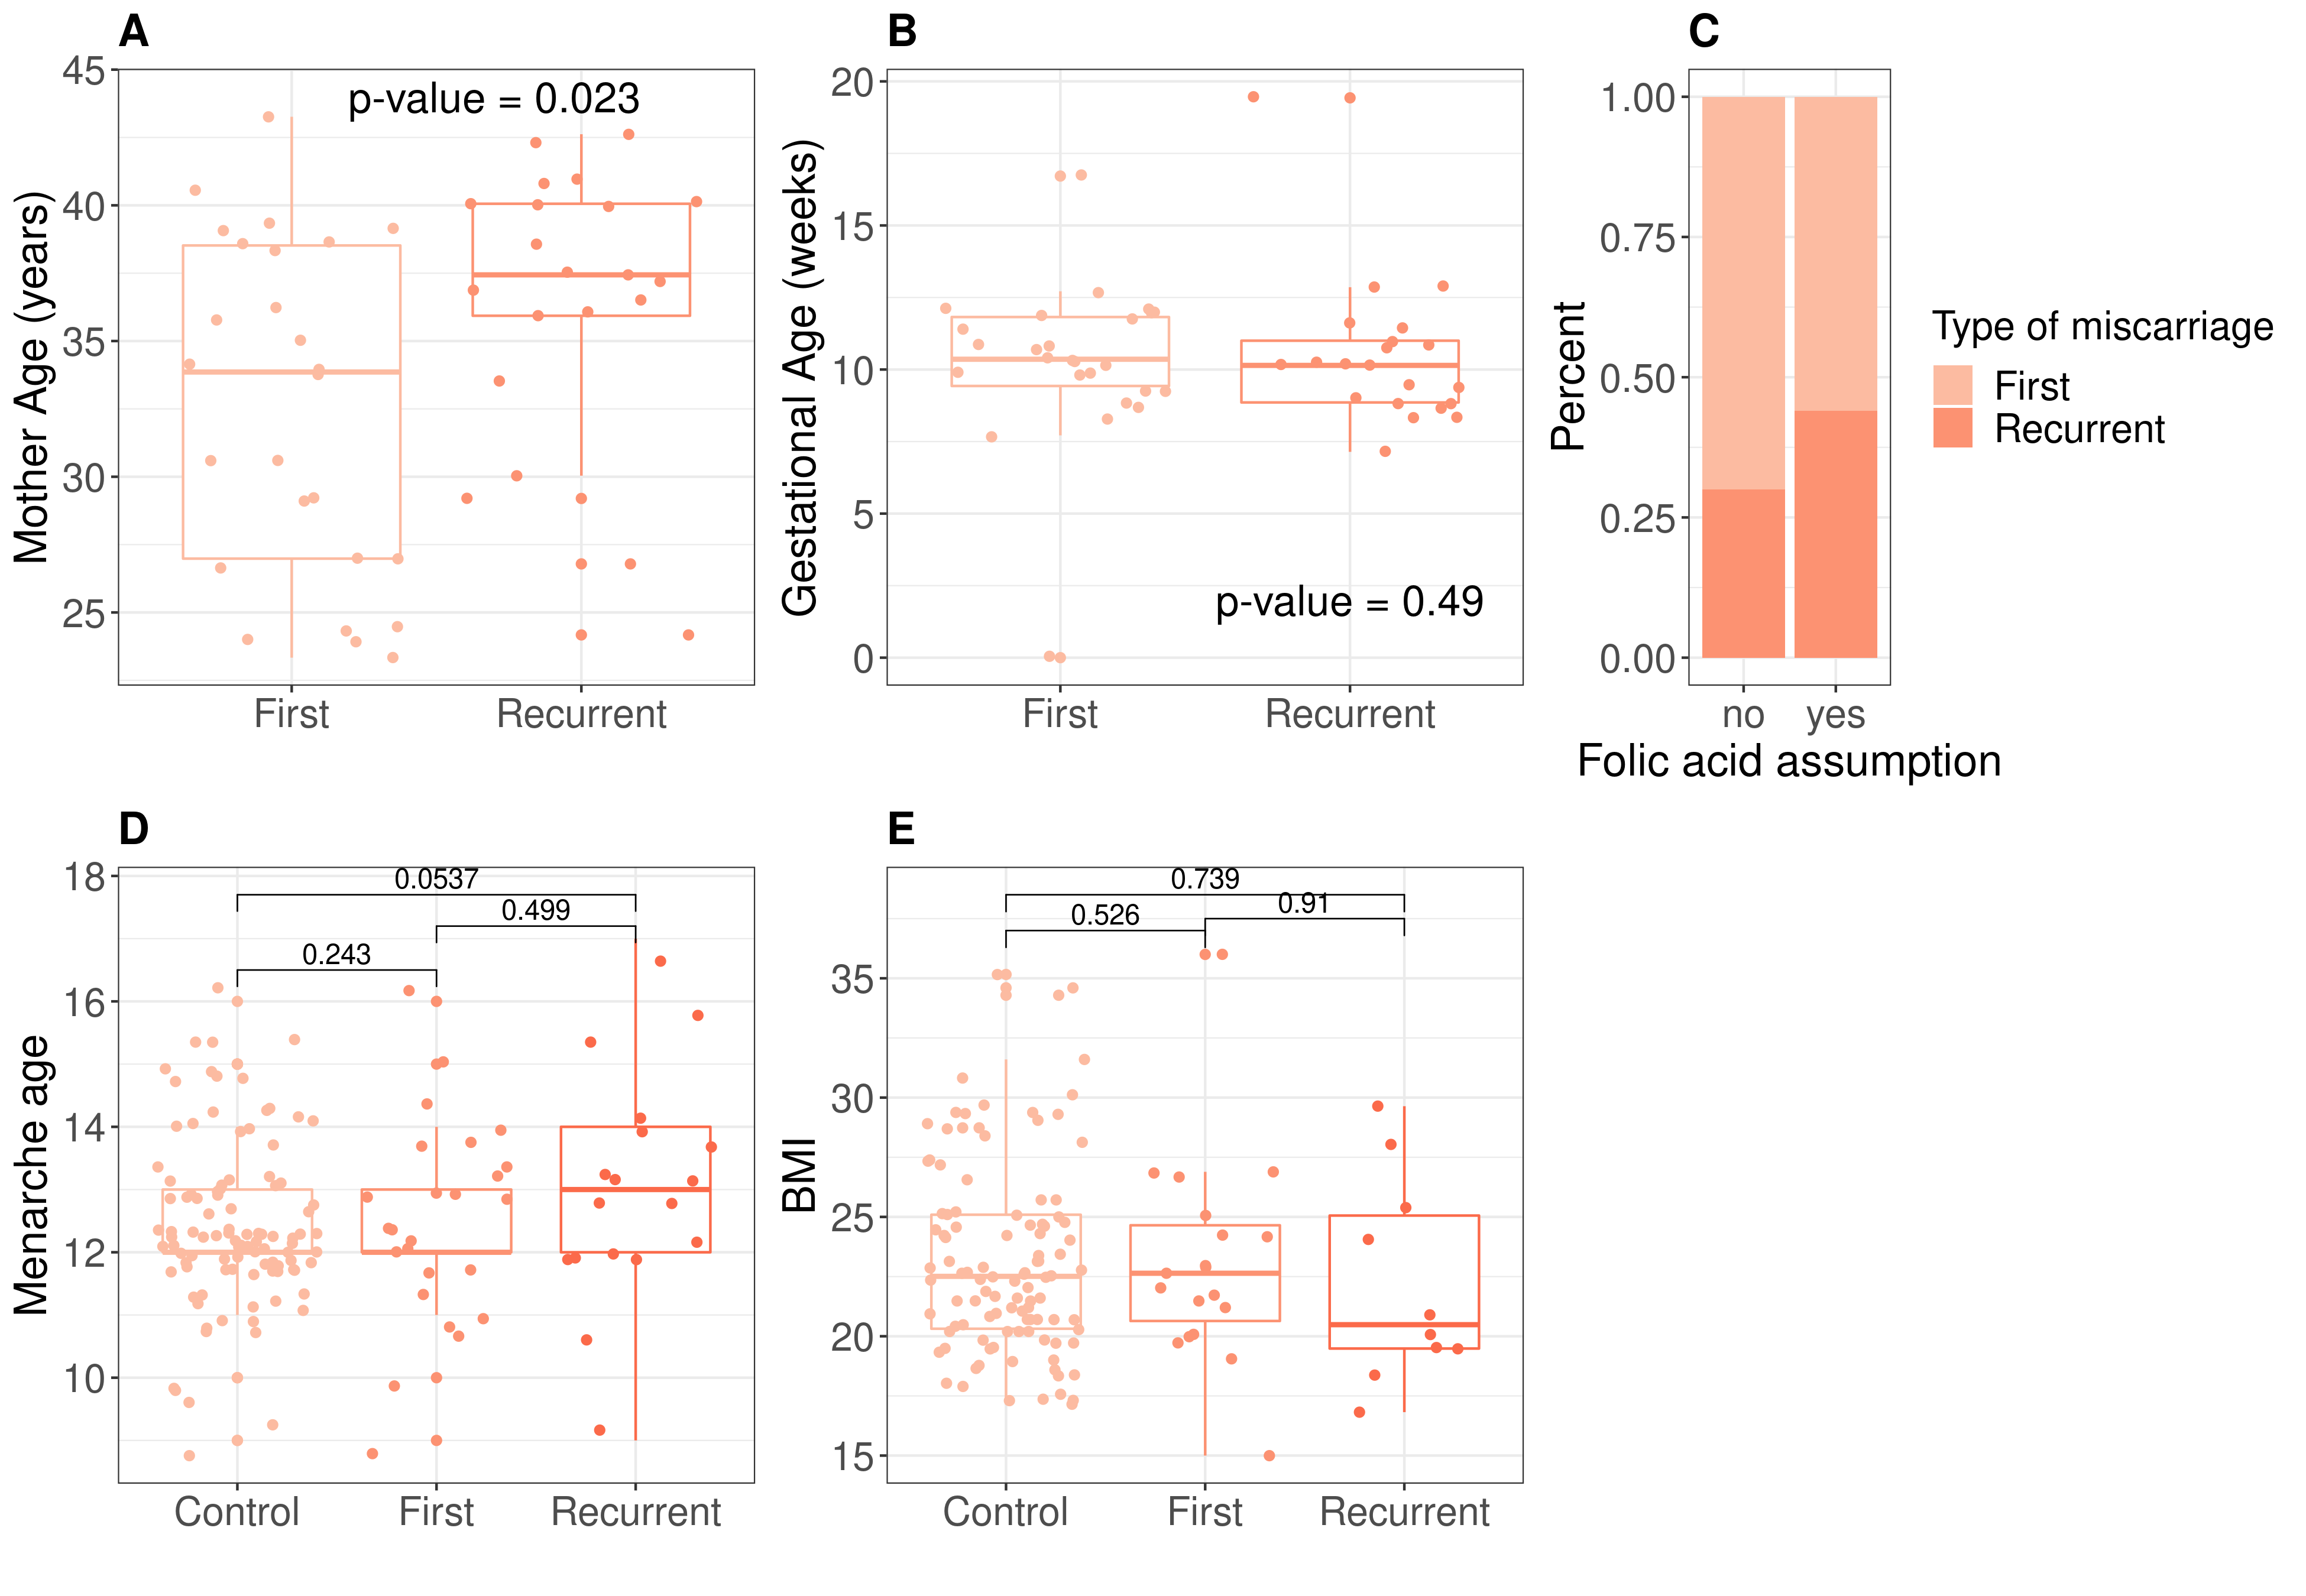
\includegraphics[width=0.7\textwidth]{Fig/panel_stats.png}
\decoRule
\caption{\textbf{Features of the embryo's mothers.} \textbf{(A)} Median age of the mother at the event for first and recurrent miscarriages, with no significant difference between the two classes. \textbf{(B)} Gestational age at the time of the pregnancy termination with no significant difference between first and recurrent cases.  \textbf{(C)} Folic acid intake. Range of values of menarche age \textbf{(D)} and Body Mass Index \textbf{(E)} in embryo's mothers are not significantly different from a control set of mothers undergoing voluntary termination of pregnancy.}
\label{fig:mothers}
\end{figure}


%%%%%%%%%%%%%%%%%%%%%%%%%%%%%%%%%%%%%%%%%%%%%%%%%%%%%%%%%%%
%  Section 
%%%%%%%%%%%%%%%%%%%%%%%%%%%%%%%%%%%%%%%%%%%%%%%%%%%%%%%%%%%

\section{Characterization of variants in the mitochondrial DNA}




\subsection{Identification of variants}
The sequencing process produces sequence data in the \gls{fastq} format, i.e. the raw sequence data that I used to perform the variant calling analysis on high performance computing machines. %Figure \ref{fig:align-ref-vc} provides an overview of the pipeline used in this study.\newline
The variant calling is the process of identification of variants from sequence data, where variants are chunks of sequence that differ from the reference genome. Genetic variants are classified as single nucleotide variants (SNVs), small insertions and deletions (indels), and structural variants (SVs, large genomic rearrangements). (Figure \ref{fig:variantCalling})

\begin{figure}[H]
\centering
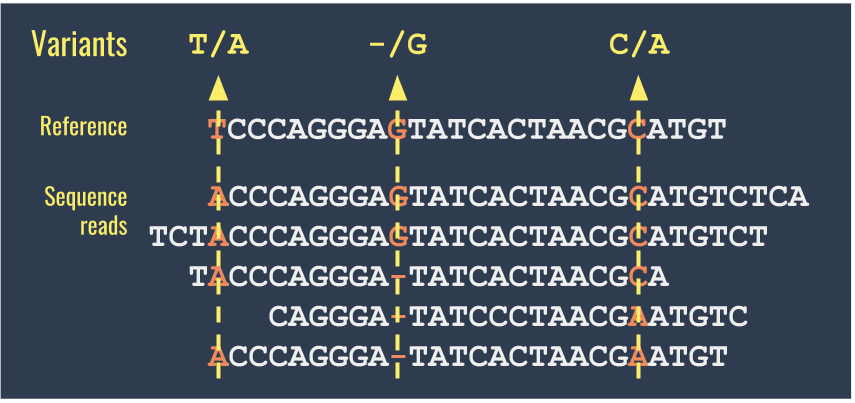
\includegraphics[width=0.7\textwidth]{Fig/variantCalling.png}
\decoRule
\caption{\textbf{Variant calling} is the process of identifying genetic variants. First, sequence reads from one individual are aligned against the reference genome, then variable sites are identified as the ones where the sequence differs from the reference genome.} 
\label{fig:variantCalling}
\end{figure}



The first step in variant calling is the \textbf{alignment} of the raw sequence data in form of reads against the most recent version of the human reference Genome (GRChg38.p12, \cite{rosenbloom2015ucsc}) using \textsc{bwa-mem} (\cite{li2013aligning}) and \textsc{samtools}. (\cite{li2009sequence}) The alignment produces files in the bam format that provide information on the quality of the alignment and enable some quality controls.  In our data set the majority of the reads were correctly aligned to the reference genome. 

Before proceeding to the next step I used \textsc{sambamba} (\cite{tarasov2015sambamba}) to \textbf{refine} the data and remove PCR duplicates, i.e. reads that came from the same DNA fragment that bias variant detection through increased homozygosity.\newline

I used the refined bam file to perform \textbf{variant calling} using \textsc{mity} (\cite{puttick2019mity}) that is based on the \textsc{freebayes} algorithm (\cite{garrison2012haplotype}). Variant calling produces data in the vcf format. 

The final step is a second round of \textbf{refining} that includes three steps. 
\begin{itemize}
    \item I used \textsc{vcffilter} (\cite{vcflib}) to filter variants for \gls{quality score}(QUAL)>30. The QUAL is an estimate of how likely it is to observe a call by chance, and a value of 30 corresponds to 1\% probability of having an incorrect genotype.
    \item I used \textsc{vt} (\cite{tan2015unified}) to do the normalization that consist of two parts: parsimony and left alignment. Parsimony is the representation of a variant in as few nucleotides as possible without reducing the length of any allele to 0. Left alignment is the shift of the start position of a variant to the left till it is no longer possible to do so (Figure \ref{fig:vtNorm}) (\cite{tan2015unified}).
    \item I used \textsc{vt} to deconstruct multiallelic variants in a VCF to allow for allelic comparisons between call sets
\end{itemize}

\begin{figure}[H]
\centering
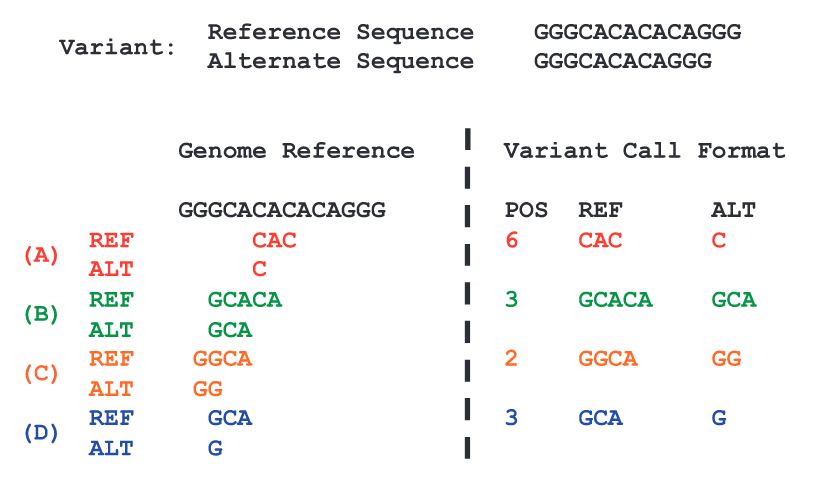
\includegraphics[width=0.65\textwidth]{Fig/vtNormalizeTan.png}
\decoRule
\caption{\textbf{Example  of  VCF  entries  representing  the  same  variant.} \textit{ Adapted from \cite{tan2015unified}}. Left  panel aligns each allele to the reference genome, and the right panel represents thevariant in VCF. (A) is not left-aligned (B) is neither left-aligned nor parsimonious, (C) is not parsimonious and (D) is normalized}
\label{fig:vtNorm}
\end{figure}

\begin{figure}[H]
\centering
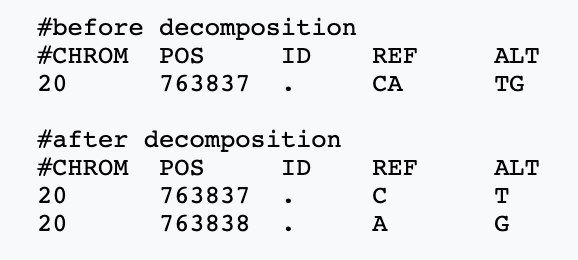
\includegraphics[width=0.5\textwidth]{Fig/vtDecompose.png}
\decoRule
\caption{\textbf{Decomposes biallelic clumped variant} for allelic comparisons between call sets} \textit{ Adapted from \cite{tan2015unified}}. 
\label{fig:vtDecomp}
\end{figure}

Overall, the variant calling with \textsc{mity} identified 276 unique variable sites of which 44 are in the D-Loop (positions 309-566) that is more variable than the rest of the mitochondrial DNA as expected (\cite{chinnery2014mitochondrial}). In particular there is one variable sites every 5.8 bp in the D-loop \textit{versus} 70.3 bp in the rest of DNA.\\


\begin{figure}[H]
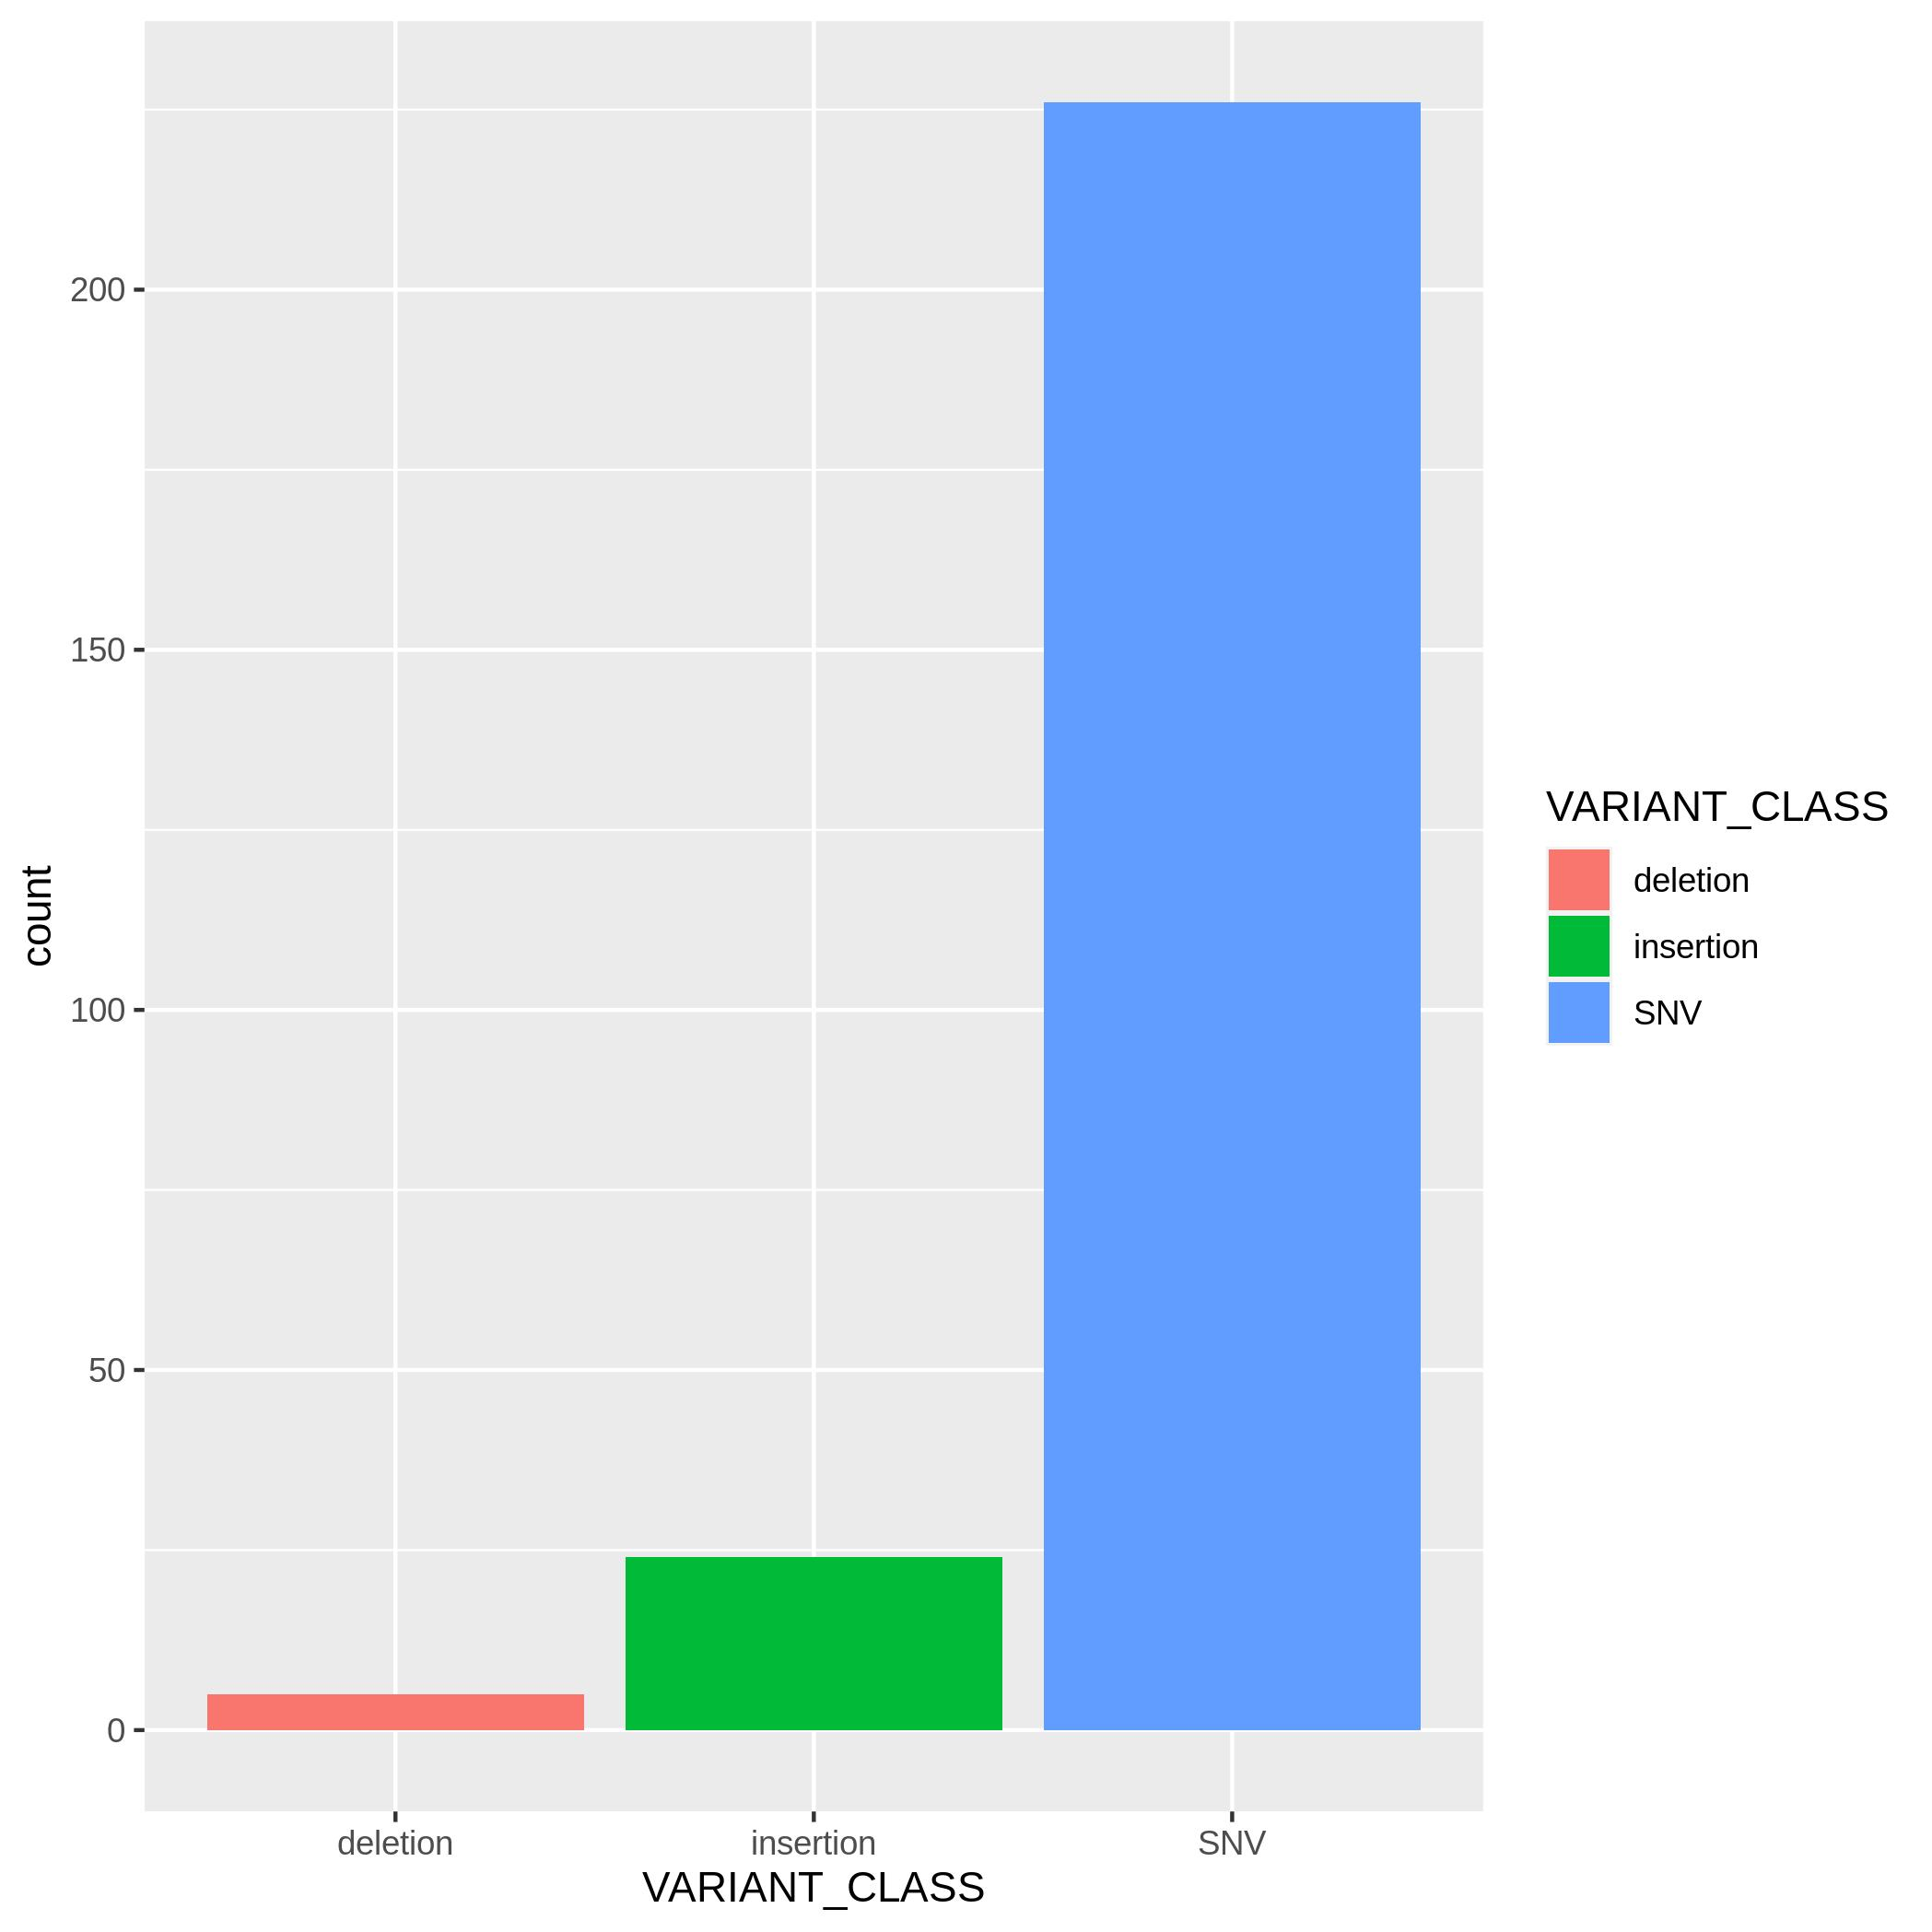
\includegraphics[width=8cm]{Fig/VC_vep_deco.jpg}
\caption{Classes of variants in the mitochondrial DNA of the ten embryos}
\label{fig:variantclass}
\end{figure}



There are three classes of variants in the mitochondrila data set of the ten embryos (Figure \ref{fig:variantclass}): deletion (n=6), insertion (n=30) and SNV (n=240).
%Variant classes 



Per each sample, the number of variable sites vary between 22 and 103 (Table \ref{tab:stats_variantcalling}). On average, the majority (90\%) of the variants is Single Nuclotide Variants. The other types of variants are indels.\\

{\begin{table}[H]
\caption{Variant classes count per sample}
\label{tab:stats_variantcalling}
\centering
\begin{tabular}{1 1 1}
\toprule
\tabhead{ID} & \tabhead{SNV} & \tabhead{InDels}   \\
\midrule
AS006 & 22 & 5  \\
AS030 & 18 & 4  \\
AS036 & 28 & 1  \\
AS054 & 94 & 9   \\
AS064 & 17 & 3   \\
AS065 & 61 & 5  \\
AS074 & 22 & 2  \\
AS087 & 46 & 1  \\
AS090 & 41 & 3   \\
AS093 & 45 & 1  \\
AS094 & 47 & 7   \\
\bottomrule\\
\end{tabular}
\end{table}
}
 

%%%%%%%%%%%%%%%%%%%%%%%%%%%%%%%%%%%%%
\subsection{Functional annotations of variants}

The  Variant Effect Predictor (VEP) software determines the effect of variants (SNPs, insertions, deletions, CNVs or structural variants) on genes, transcripts, and protein sequence, as well as regulatory regions (\cite{mclaren2016ensembl}). Table \ref{tab:csqVEP} (adapted from \cite{mclaren2016ensembl}) describes the classification of the consequences in the Ensembl Variation data base.
%blocca a tabella qui se ci riesci
{\small
\begin{sidewaystable}[H]
\caption{Table of Consequences}
\label{tab:csqVEP}
\centering
\begin{adjustbox}{width=1\textwidth}
\begin{tabular}{c c c c}
\toprule
\tabhead{SO term} & \tabhead{SO description} & \tabhead{SO accession} & \tabhead{Impact} \\
\midrule
transcript ablation & A feature ablation whereby the deleted region includes a transcript feature & SO:0001893 & HIGH \\
splice acceptor variant & A splice variant that changes the 2 base region at the 3' end of an intron & SO:0001574 & HIGH \\
splice donor variant & A splice variant that changes the 2 base region at the 5' end of an intron & SO:0001575 & HIGH \\
stop gained & A sequence variant whereby at least one base of a codon is changed, resulting in a premature stop codon, leading to a shortened transcript & SO:0001587 & HIGH \\
frameshift variant & A sequence variant which causes a disruption of the translational reading frame, because the number of nucleotides inserted or deleted is not a multiple of three & SO:0001589 & HIGH \\
stop lost & A sequence variant where at least one base of the terminator codon (stop) is changed, resulting in an elongated transcript & SO:0001578 & HIGH \\
start lost & A codon variant that changes at least one base of the canonical start codon & SO:0002012 & HIGH \\
transcript amplification & A feature amplification of a region containing a transcript & SO:0001889 & HIGH \\
inframe insertion & An inframe non synonymous variant that inserts bases into in the coding sequence & SO:0001821 & MODERATE \\
inframe deletion & An inframe non synonymous variant that deletes bases from the coding sequence & SO:0001822 & MODERATE \\
missense variant & A sequence variant, that changes one or more bases, resulting in a different amino acid sequence but where the length is preserved & SO:0001583 & MODERATE \\
protein altering variant & A sequence variant which is predicted to change the protein encoded in the coding sequence & SO:0001818 & MODERATE \\
splice region variant & A sequence variant in which a change has occurred within the region of the splice site, either within 1-3 bases of the exon or 3-8 bases of the intron & SO:0001630 & LOW \\
incomplete terminal codon variant & A sequence variant where at least one base of the final codon of an incompletely annotated transcript is changed & SO:0001626 & LOW \\
start retained variant & A sequence variant where at least one base in the start codon is changed, but the start remains & SO:0002019 & LOW \\
stop retained variant & A sequence variant where at least one base in the terminator codon is changed, but the terminator remains & SO:0001567 & LOW \\
synonymous variant & A sequence variant where there is no resulting change to the encoded amino acid & SO:0001819 & LOW \\
coding sequence variant & A sequence variant that changes the coding sequence & SO:0001580 & MODIFIER \\
mature miRNA variant & A transcript variant located with the sequence of the mature miRNA & SO:0001620 & MODIFIER \\
5 prime UTR variant & A UTR variant of the 5' UTR & SO:0001623 & MODIFIER \\
3 prime UTR variant & A UTR variant of the 3' UTR & SO:0001624 & MODIFIER \\
non coding transcript exon variant & A sequence variant that changes non-coding exon sequence in a non-coding transcript & SO:0001792 & MODIFIER \\
intron variant & A transcript variant occurring within an intron & SO:0001627 & MODIFIER \\
NMD transcript variant & A variant in a transcript that is the target of NMD & SO:0001621 & MODIFIER \\
non coding transcript variant & A transcript variant of a non coding RNA gene & SO:0001619 & MODIFIER \\
upstream gene variant & A sequence variant located 5' of a gene & SO:0001631 & MODIFIER \\
downstream gene variant & A sequence variant located 3' of a gene & SO:0001632 & MODIFIER \\
TFBS ablation & A feature ablation whereby the deleted region includes a transcription factor binding site & SO:0001895 & MODIFIER \\
TFBS amplification & A feature amplification of a region containing a transcription factor binding site & SO:0001892 & MODIFIER \\
TF binding site variant & A sequence variant located within a transcription factor binding site & SO:0001782 & MODIFIER \\
regulatory region ablation & A feature ablation whereby the deleted region includes a regulatory region & SO:0001894 & MODERATE \\
regulatory region amplification & A feature amplification of a region containing a regulatory region & SO:0001891 & MODIFIER \\
feature elongation & A sequence variant that causes the extension of a genomic feature, with regard to the reference sequence & SO:0001907 & MODIFIER \\
regulatory region variant & A sequence variant located within a regulatory region & SO:0001566 & MODIFIER \\
feature truncation & A sequence variant that causes the reduction of a genomic feature, with regard to the reference sequence & SO:0001906 & MODIFIER \\
intergenic variant & A sequence variant located in the intergenic region, between genes & SO:0001628 & MODIFIER \\
\bottomrule\\
\end{tabular}
\end{adjustbox}
\end{sidewaystable}
}



%Most severe consequence
I run VEP on the vcf files obtained from the variant calling. The VEP software identifies the most severe consequence for the given variants. In our DNA sequences VEP classifies the majority as upstream gene variants (255), 84 as synonymous variant, 46 as missense variant, and 33 are non coding transcript exon variant.
(Figure \ref{Fig:Vep Consequence})


\begin{figure}[H]
\centering
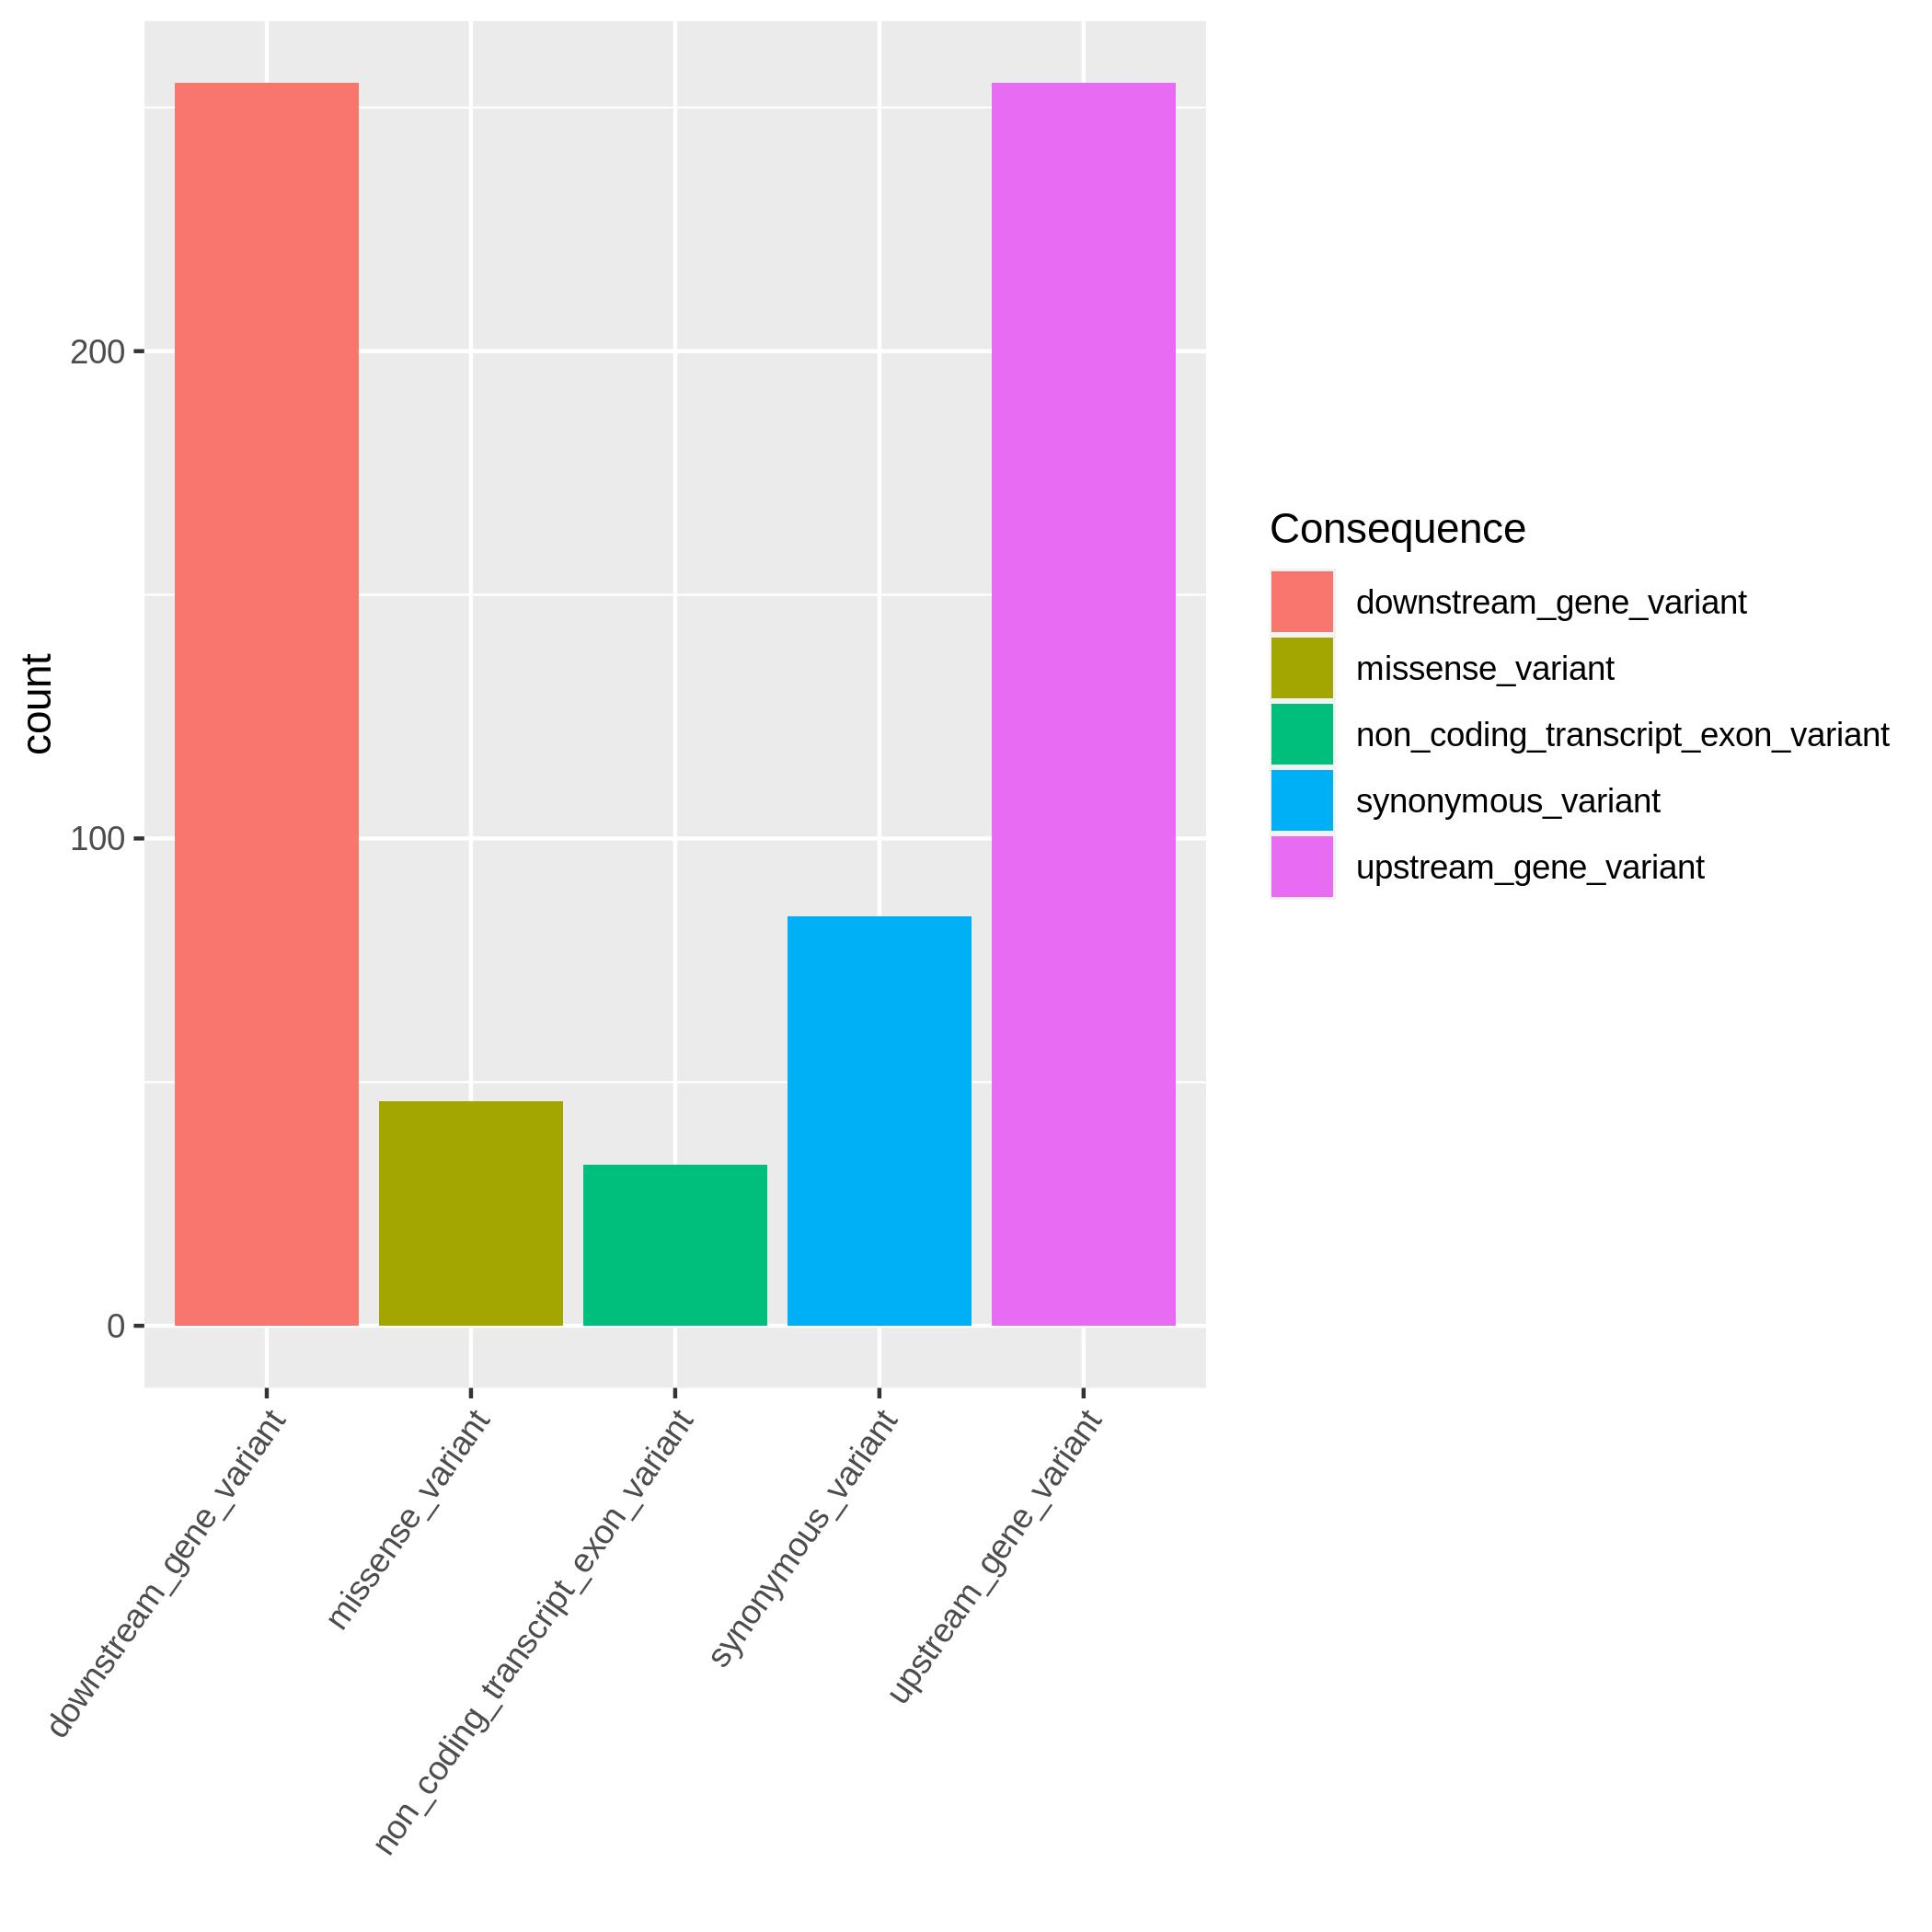
\includegraphics[width=0.65\textwidth]{Fig/VepConseguence_decom_plot.jpg}
\decoRule
\caption{\textbf{Classification of mitochondrial variants according to VEP.}}
\label{Fig:Vep Consequence}
\end{figure}

Among variants in the coding consequences there are synonymous and missense. Synonymous mutations on the DNA sequence result in the same amino acid, therefore they are considered of low impact. Missense variants are instead considered of high impact because their effect is to change the amino acid in the protein coded by the gene therefore, missense variants can alter the function of the protein. For the missense variants, VEP annotates also SIFT and PolyPhen scores. SIFT predicts whether an amino acid substitution affects protein function based on sequence homology and the physical properties of amino acids (\cite{ng2003sift}). The SIFT score ranges from 0.0 (deleterious) to 1.0 (tolerated). In my samples there are 21 variants defined as tolerated with low confidence, 13 deleterious with low confidence, 8 tolerated variants and 4 deleterous (Figure \ref{fig:siftpolyphen}).
 
The PolyPhen score predicts the possible impact of an amino acid substitution on the structure and function of a human protein \cite{adzhubei2013predicting}.The PolyPhen score ranges from 0.0 (tolerated) to 1.0 (deleterious). Variants with scores of 0.0 are predicted to be benign. Values closer to 1.0 are more confidently predicted to be deleterious. In my samples I find 28 benign variants, 15 probably damaging variants, 2 possibly damaging variants and 1 unknown (Figure \ref{fig:siftpolyphen}).\\

%figura 
\begin{figure}[H]
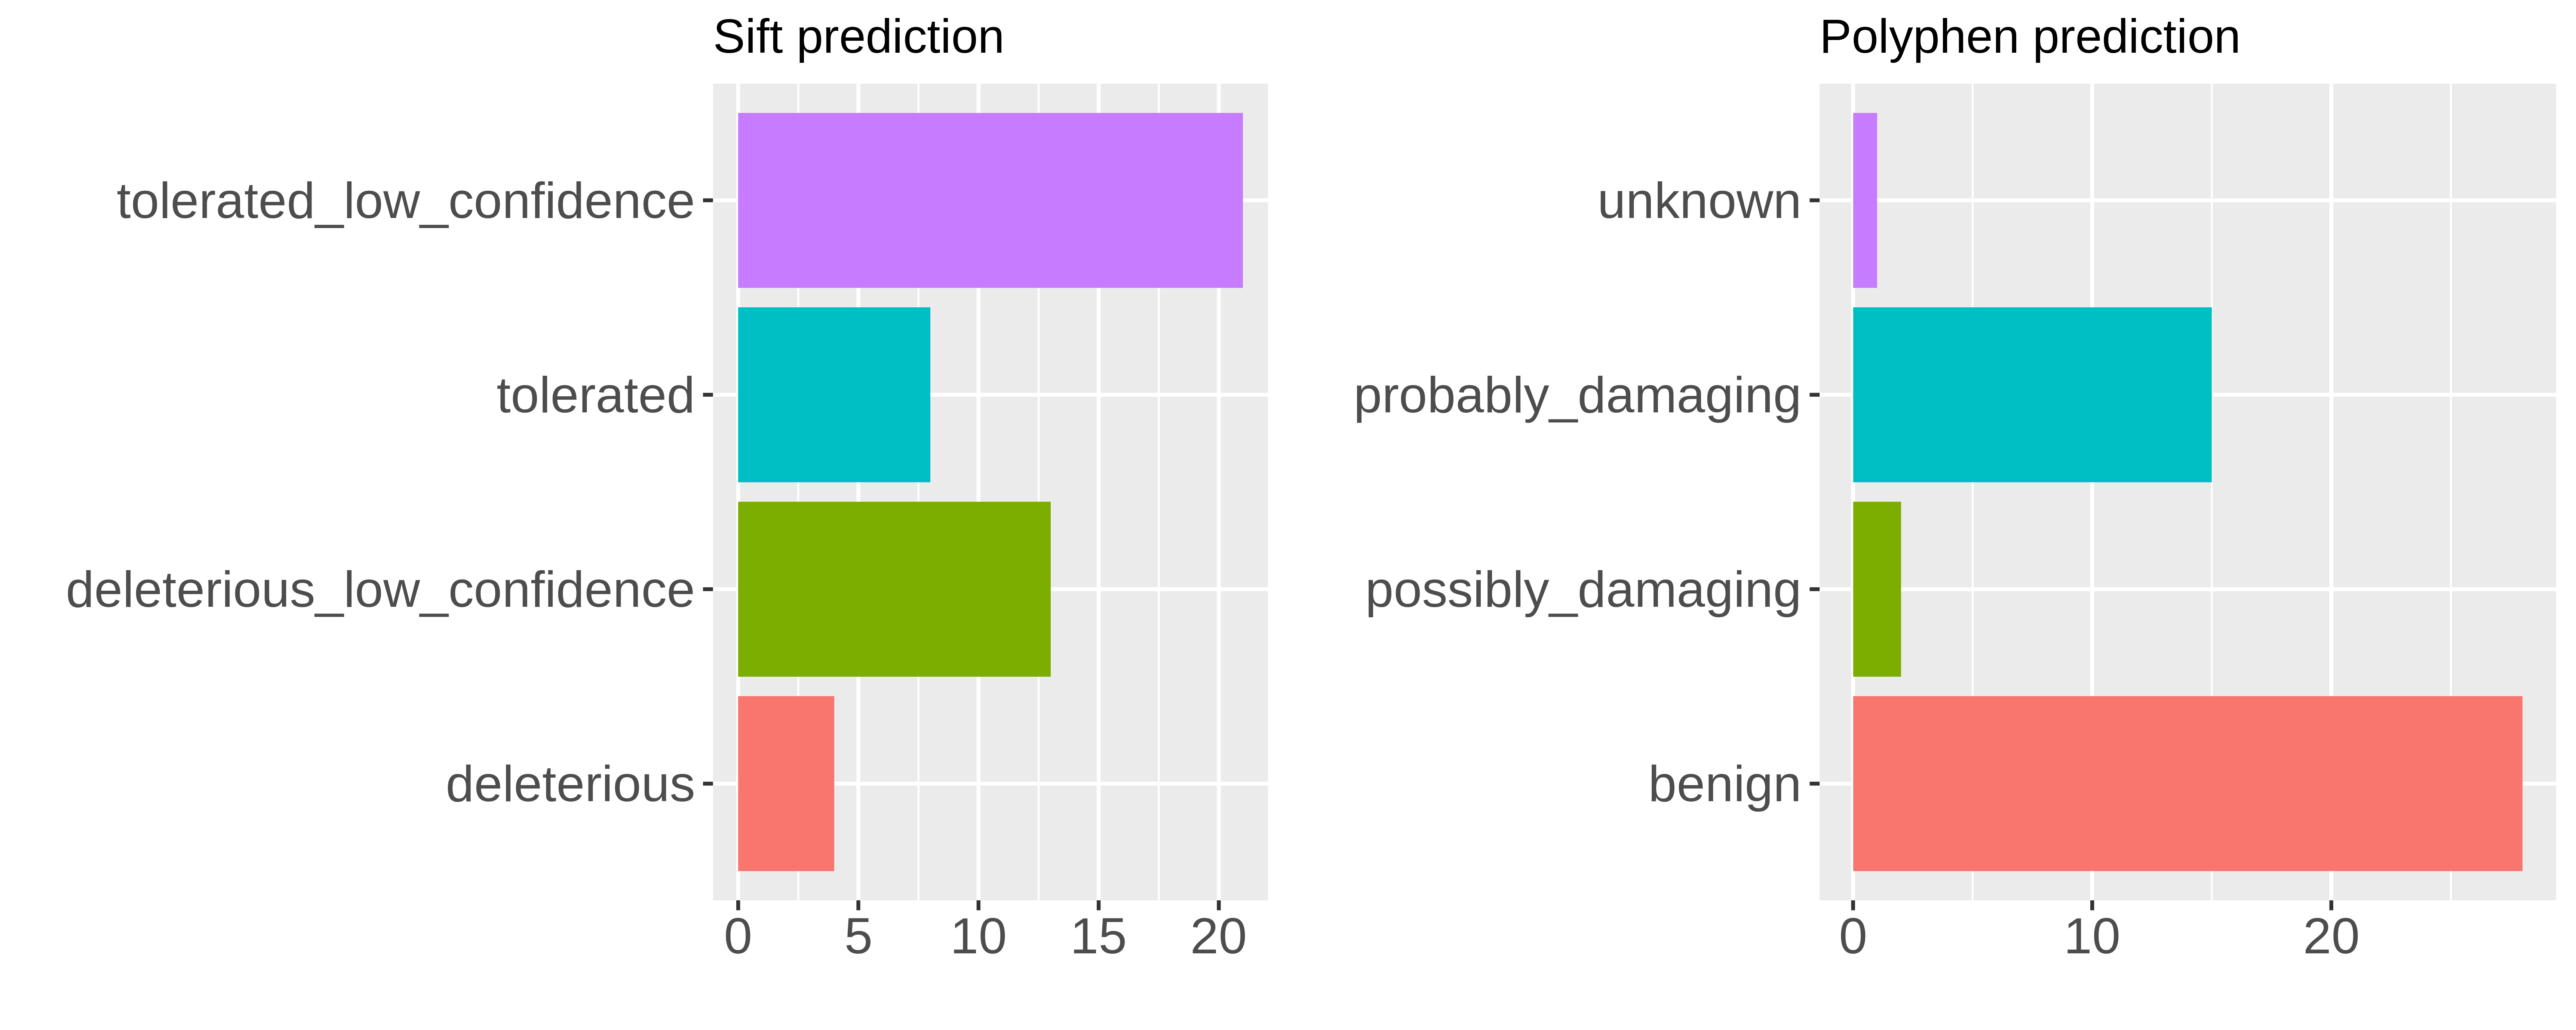
\includegraphics[width=\textwidth]{Fig/plots2.png}
\caption{Sift and Polyphen}
\label{fig:siftpolyphen}
\end{figure}\\

Three of the four deleterious variants identified by SIFT are novel, i.e. are found only in these samples  described in Table \ref{tab:missense}. % The variants are located at positions "5374" with PolyPhen  benign with a score of 0.253, "8668" with PolyPhen probably damaging with a score of 0.947, "14447" with PolyPhen possibly damaging with a score of 0.861 and at position"14556" with PolyPhen probably damaging with score 0.999. 
These variants are found in the \textit {MT-ND2}, \textit{MT-ATP6} and
\textit{MT-ND6} genes and are shared by more than one sample (Table \ref{tab:missenseDel0.genotypes}). In particular the variant at position 14556 in the \textit{MT-ND6} gene is shared by 8 samples. 


\textit{MT-ND2} is a mitochondrial gene coding for the NADH dehydrogenase 2 (ND2) protein.The ND2 protein is a subunit of NADH dehydrogenase (ubiquinone), which is located in the mitochondrial inner membrane and is the largest of the five complexes of the
electron transport chain (\cite{ncbi2016database}). \textit{MT-ATP6} (or ATP6) is a mitochondrial gene that encodes the ATP synthase Fo subunit 6 (or subunit/chain A).This subunit belongs to the Fo complex of the complex V. This enzyme is responsible for the final step of oxidative phosphorylation in the electron transport chain (\cite{ncbi2016database}). 


\textit{MT-ND6} is a mitochondrial gene coding for the NADH-ubiquinone oxidoreductase chain 6 protein (ND6). The ND6 protein is a subunit of NADH dehydrogenase (ubiquinone), which is located in the mitochondrial inner membrane and is the largest of
the five complexes of the electron transport chain (\cite{ncbi2016database}).



%rs non riportati

{\small
\begin{table}[H]
\caption{Missense Variants classified as deleterius according to SIFT and PolyPhen }
\label{tab:missense}
\centering
\begin{adjustbox}{width=1\textwidth}
\begin{tabular}{c c c c c c c}
\toprule
\tabhead{Location chrM} & \tabhead{Variation Allele} &
\tabhead{existing Variation} & \tabhead{Codons} & \tabhead{SYMBOL} & \tabhead{SIFT (score)} & \tabhead{PolyPhen (score)} \\
\midrule
5374 & T/C  & - & aTc/aCc & \textit{MT-ND2} & deleterious (0) &  benign (0.253)   \\%ENSG00000198763
8668 & T/C &  COSV62293167 & Tga/Cga & \textit{MT-ATP6} & deleterious (0)&      probably damaging (0.997)   \\ %ENSG00000198899
14447 & T/C & - & gAg/gGg & \textit{MT-ND6} & deleterious (0) &     possibly damaging (0.861) \\ %ENSG00000198695
14556 & A/C & - & Tgt/Ggt & \textit{MT-ND6} & deleterious (0) &      probably damaging (0.999)   \\ %ENSG00000198695
\bottomrule\\
\end{tabular}
\end{adjustbox}
\end{table}
}

Pathogenic variants of the mitochondrial gene \textit{MT-ND2} are known to cause mtDNA-associated Leigh syndrome, as are variants of \textit{MT-ATP6} and \textit{MT-ND6}. Abnormalities in mitochondrial energy generation result in neurodegenerative disorders like Leigh syndrome, which is characterized by an onset of symptoms between 12 months and three years of age. The symptoms frequently present themselves following a viral infection and include movement disorders and peripheral neuropathy, as well as hypotonia, spasticity and cerebellar ataxia. Roughly half of affected patients die of respiratory or cardiac failure by the age of three. Leigh syndrome is a maternally inherited disorder and its diagnosis is established through genetic testing of the aforementioned mitochondrial genes
(\cite{thorburn2017mitochondrial}). 


{\small
\begin{table}[H]
\caption{Genotypes of missense variants in the embryos.}
\label{tab:missenseDel0.genotypes}
\centering
\begin{tabular}{c c c c c c c}
\toprule
\tabhead{Sample ID} & \tabhead{5374} & \tabhead{8668} & \tabhead{14447} & \tabhead{14556}\\
\midrule 
AS006   &      0   &    0   &    0   &    1\\
AS030   &      0   &    0   &    0   &    0\\
AS036   &      1   &    0   &    1   &    1\\
AS054   &      1   &    1   &    1   &    1\\
AS064   &      0   &    0   &    0   &    1\\
AS065   &      0   &    0   &    1   &    0\\
AS074   &      0   &    0   &    0   &    0\\
AS087   &      1   &    0   &    0   &    1\\
AS090   &      0   &    0   &    1   &    1\\
AS093   &      1   &    1   &    1   &    1\\
AS094   &      1   &    0   &    1   &    1\\
TOTAL SHARED   &     5    &    2  &     6   &    8\\
\bottomrule\\
\end{tabular}
\end{table}
}


\section{Nuclear genes involved in mitochondrial process}

After exploring variation in the mitochondrial genome, I have analyzed variation in nuclear genes whose product are involved in mitochondrial processes. First I selected these genes using gene ontology(GO). The GO database (\cite{ashburner2000gene}) is a collection of structured vocabularies, or ontologies, that describe and relate gene products in terms of their biological properties. In GO I found 1,384 genes involved in mitochondrial process. 


I then run the \textsc{VEP} analysis to annotate the 766,845 variants found in the 1,384 genes that are presents in the ten genomes of the embryos and the results are summarized in Figure (\ref{fig:mostsevereconsequence}), stratified by four categories of impact: High, Modifier, Moderate, and Low. The majority of variants are intronic with modifier impact. There are 65 variants with moderate effect and nine variants with high impact.  
Among the variants with high impact the most frequent type is splice acceptor, followed by splice donor and frameshift (Table \ref{tab:MostSevereConsequence}). 
 

\begin{figure}[h]
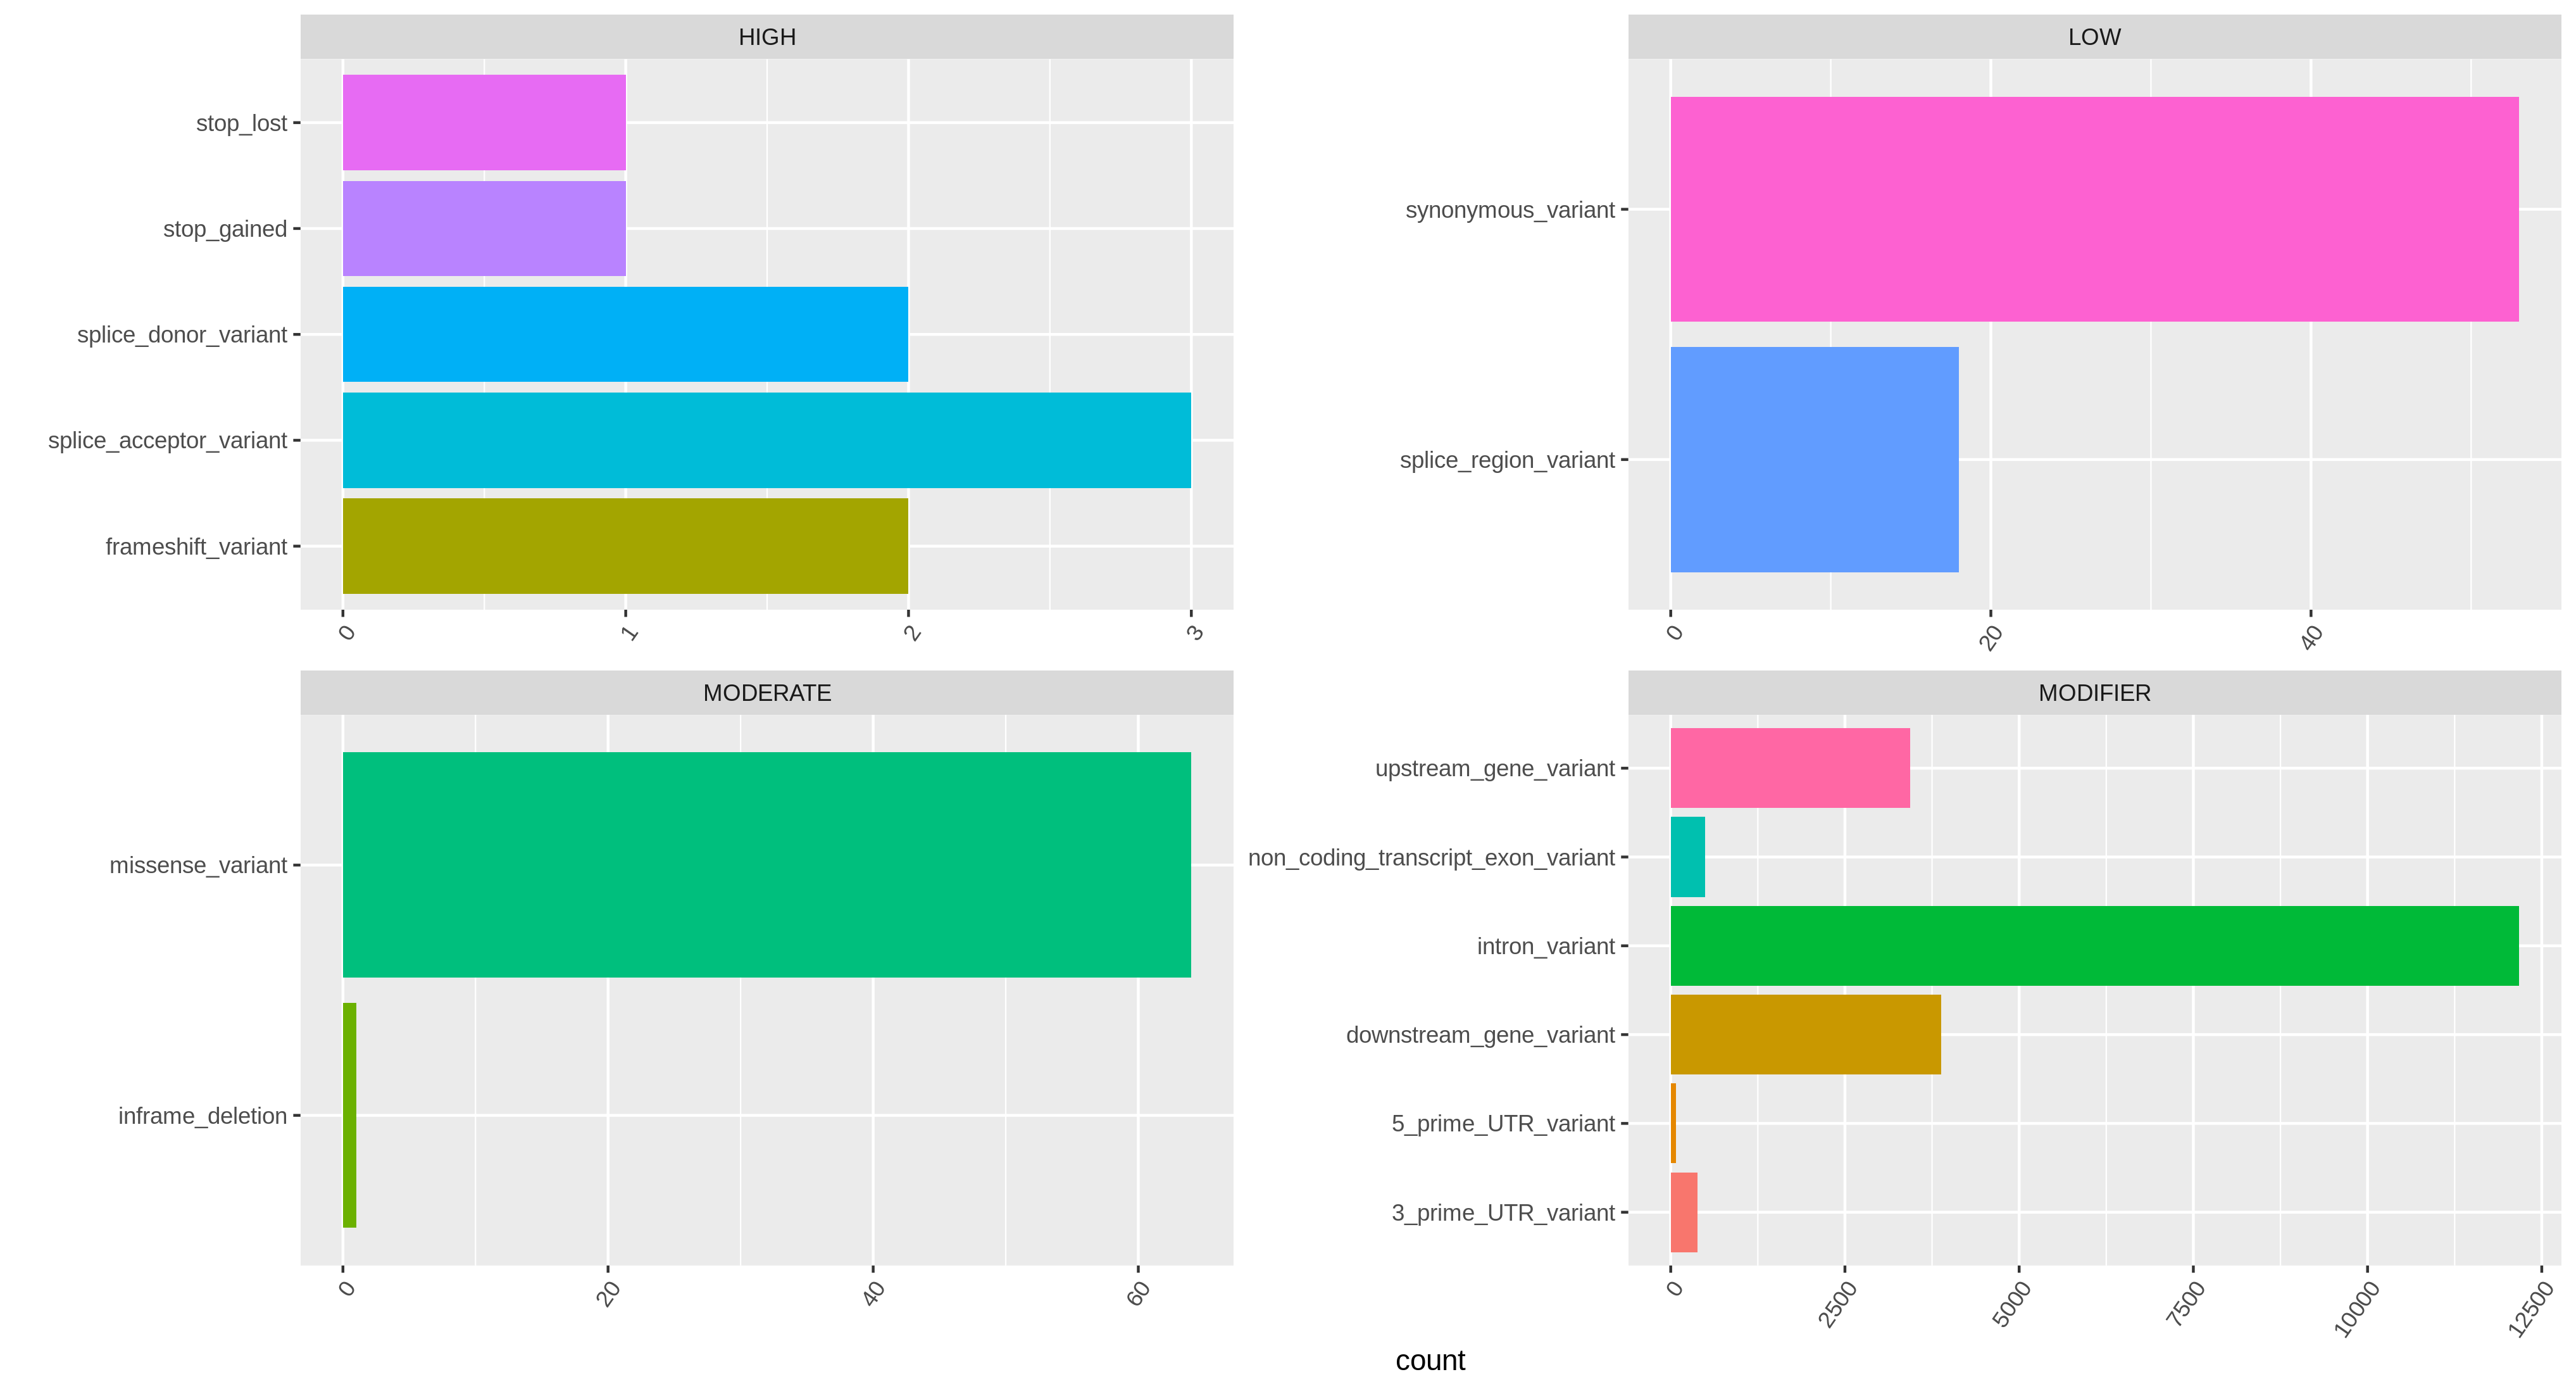
\includegraphics[width=\textwidth]{Fig/consequence.png}

\caption{Most severe consequence of variants according to VEP in the nuclear genes expressed in the mitochondria}
\label{fig:mostsevereconsequence}
\end{figure}\\


{\small
\begin{table}[H]
\caption{Variants in nuclear genes expressed in the mitochondrial that have high-impact consequences. Missense variants are excluded and reported in detail in Table \ref{tab:SiftDeleterious} and Table \ref{tab:PolyphenDeleterious}}
\label{tab:MostSevereConsequence}
\centering
\begin{adjustbox}{width=1\textwidth}
\begin{tabular}{c c c c c}
\toprule
\tabhead{Location} & \tabhead{Variation Allele}  & \tabhead{Symbol} & \tabhead{consequence} & \tabhead{Existing variation} \\
\midrule
chr10:133554659 & A/G &  \textit{CYP2E1} & non coding transcript variant & rs2149616 \\                                 
chr6:36986144 &  G/- &  \textit{MTCH1} & frameshift variant & rs35538959 \\                              
chr3:119503609 & G/C   &  \textit{TIMMDC1} & NMD transcript variant & rs1131265 \\                            
chr3:139349435 & G/A  &  \textit{MRPS22}  & NMD transcript variant & rs10935321\\                          
chr6:131547079 & A/G   &  \textit{ARG1}  & non coding transcript variant & rs2781646 \\                                
chr17:14102122 & G/A  &  \textit{COX10} & NMD transcript variant & rs2159132\\
chr10:50002097 & G/A  & \textit{TIMM23B-AGAP6} & non coding transcript variant & rs565737328 \\
chr14:70359741 & T/G &  \textit{SYNJ2BP-COX16} & NMD transcript variant & rs17475333 \\
chr14:70049036 & T/- &  \textit{SLC8A3} & frameshift variant & NA \\
\bottomrule\\
\end{tabular}
\end{adjustbox}
\end{table}
}



{\small
\begin{table}[H]
\caption{Genotype of embryos at nuclear loci with high impact consequences reported in Table \ref{tab:MostSevereConsequence} }
\label{tab.high impact genotypes}
\begin{adjustbox}{width=1\textwidth}
\centering
\begin{tabular}{c c c c c c c c c c c c}
\toprule
\tabhead{Existing variation} & \tabhead{AS006} & \tabhead{AS030} & \tabhead{AS036} & \tabhead{AS054}  & \tabhead{AS064} & \tabhead{AS065} & \tabhead{AS087} & \tabhead{AS090} & \tabhead{AS093} & \tabhead{AS094} & \tabhead{SYMBOL} \\
\midrule 
rs2149616  & 1   &   0    &  0  &    0  &    0   &   1  &    0   &   0   &   2   &   0     & \textit{CYP2E1} \\
rs565737328  & 0    &  0     & 0   &   1   &   0    &  0   &   0    &  0   &   0   &   0     & \textit{TIMM23B-AGAP6}\\
rs17475333  & 0    &  0     & 0  &    0  &    1   &   1   &   0    &  0  &    0   &   0     & \textit{SYNJ2BP-COX16}\\
rs2159132  & 1    &  0    &  1  &    2  &    1   &   1   &   0    &  2  &    1   &   0    &  \textit{COX10}\\
rs1131265 & 0    &  1    &  0  &    0  &    0   &   0   &   1   &   0  &    1   &   0    &  \textit{TIMMDC1}\\
rs10935321 & 0    &  0    &  1  &    0  &    2    &  0   &   1   &   1  &    0   &   2  &   \textit{MRPS22}\\
rs2781646 & 1   &   0    &  0   &   1   &   0   &   0   &   1   &   0  & 0   &   1  &    \textit{ARG1}\\

\bottomrule\\
\end{tabular}
\end{adjustbox}
\end{table}
}

\subsection{High-impact stop gain mutation in the nuclear gene \textit{COX10} and splice donor variant in the nuclear gene \textit{MRPS22}}  

Table \ref{tab.high impact genotypes} shows that the high-impact stop gain variant rs2159132 in the Cytochrome c oxidase assembly factor heme A:farnesyltransferase (\textit{COX10}) gene is the most frequent variant among embryos being shared by 7 samples. rs2159132 variant is considered by SIFT as deleterious with a 0 score and by PolyPhen as possibly damaging with a 0.63 score. Cytochrome c oxidase (COX), the terminal component of the mitochondrial respiratory chain, catalyzes the electron transfer from reduced cytochrome c to oxygen. This component is a heteromeric complex consisting of 3 catalytic subunits encoded by mitochondrial genes and multiple structural subunits encoded by nuclear genes. The mitochondrially-encoded subunits function in electron transfer, and the nuclear-encoded subunits may function in the regulation and assembly of the complex.
Deficiencies in the activity of cytochrome c oxidase (COX) are an important cause of autosomal recessive respiratory chain disorders, such as Leigh Syndrome and hypertrophic cardiomyopathy(\cite{antonicka2003mutations}).\\ 


The splice donor variant rs10935321 in the Mitochondrial ribosomal
protein S22 (\textit{MRPS22}) it is shared by 5 embryos (Table
\ref{tab.high impact genotypes} ).
Mammalian mitochondrial ribosomal proteins are encoded by nuclear
genes and help the protein synthesis within the mitochondrion.
Mitochondrial ribosomes (mitoribosomes) consist of a small 28S
subunit and a large 39S subunit. \textit{MRPS22} encodes a 28S
subunit of the mitoribosomes.

\textit{MRPS22} is critical for ovarian development and its study
may therefore provide insight into the pathophysiology and
treatment of ovarian dysfunction. Pathogenic variants in
\textit{MRPS22} can cause primary ovarian insufficiency (POI),
defined by the loss or dysfunction of ovarian follicles associated
with amenorrhea before the age of 40. POI is a major cause of
female infertility with a prevalence greater than 1\%
(\cite{chen2018mutations}).\\ 

\subsubsection{Other relevant nuclear genes}
Following, a brief description of the genes hosting the other high-impact variants I found in my analyses : \\

\textit{CYP2E1} - Cytochrome P450 family 2 subfamily E member 1.\\
This gene encodes a member of the cytochrome P450 superfamily of enzymes. The cytochrome P450 proteins are monooxygenases which catalyze many reactions involved in drug metabolism and synthesis of cholesterol, steroids and other lipids.\\


\textit{MTCH1} - Mitochondrial carrier 1\\
This gene encodes a member of the mitochondrial carrier family. The encoded protein is localized to the mitochondrion inner membrane and induces apoptosis independent of the proapoptotic proteins Bax and Bak.\\

\textit{TIMMDC1} - Translocase Of Inner Mitochondrial Membrane Domain-Containing Protein 1 \\
This gene encode for Translocase of inner mitochondrial membrane domain containing 1.
Chaperone protein involved in the assembly of the mitochondrial NADH:ubiquinone oxidoreductase complex (complex I). Participates in constructing the membrane arm of complex I.\\

\textit{ARG1} -  Arginase 1.\\
Arginase catalyzes the hydrolysis of arginine to ornithine and urea. At least two isoforms of mammalian arginase exist (types I and II) which differ in their tissue distribution, subcellular localization, immunologic crossreactivity and physiologic function.\\

\textit{TIMM23B} - ranslocase of inner mitochondrial membrane 23 homolog B \\
This gene encode participate in the translocation of transit peptide-containing proteins across the mitochondrial inner membrane. \\

\textit{AGAP6} - A-kinase anchor protein 6.\\
The A-kinase anchor proteins (AKAPs) are a group of structurally diverse proteins, which have the common function of binding to the regulatory subunit of protein kinase A (PKA) and confining the holoenzyme to discrete locations within the cell.
The encoded protein is highly expressed in various brain regions and cardiac and skeletal muscle. \\

\textit{SYNJ2BP} - Synaptojanin-2-binding protein.\\
This protein regulates endocytosis of activin type 2 receptor kinases through the Ral/RALBP1-dependent pathway and may be involved in suppression of activin-induced signal transduction. \\


\textit{COX16} - COX16, cytochrome c oxidase assembly homolog\\
Required for the assembly of the mitochondrial respiratory chain complex IV (CIV), also known as cytochrome c oxidase. Promotes the insertion of copper into the active site of cytochrome c oxidase subunit II (MT-CO2/COX2). Interacts specifically with newly synthesized MT-CO2/COX and its copper center-forming metallochaperones SCO1, SCO2 and COA6. Probably facilitates MT-CO2/COX2 association with the MITRAC assembly intermediate containing MT-CO1/COX1, thereby participating in merging the MT-CO1/COX1 and MT-CO2/COX2 assembly lines \\

\textit{SLC8A3} - Solute carrier family 8 member A3\\
This protein is a member of the sodium/calcium exchanger integral membrane protein family. Na+/Ca2+ exchange proteins are involved in maintaining Ca2+ homeostasis in a wide variety of cell types.\\

\subsection{Moderate-impact missense variant in \textit{GMF2} }

Almost all variants with moderate impact (65 out of 766,845) are missense variants. For the missense variants, \textsc{vep} annotates also SIFT and PolyPhen scores. The SIFT score ranges from 0.0 (deleterious) to 1.0 (tolerated). The PolyPhen score ranges from 0.0 (tolerated) to 1.0 (deleterious). \\


{\small
\begin{table}[H]
\caption{Deleterious missense variants in nuclear genes expressed in mitochondria according to SIFT}
\label{tab:SiftDeleterious}
\centering
\begin{tabular}{c c c c c c c}
\toprule
\tabhead{Existing variation} & \tabhead{Position} & \tabhead{Variation} &\tabhead{Gene} \\
\midrule 
rs41304800 & chr20:3147932 & A/C & \textit{FASTKD5} \\
rs2230351 & chr17:14076741 & A/T  & \textit{COX10} \\
rs2072279 & chr17:14077033 & G/A & \textit{COX10} \\ %COX10 
rs2293925 & chr8:143310198 &  G/A  & \textit{TOP1MT} \\
\bottomrule\\
\end{tabular}
\end{table}
}

In my analysis I find 4 deleterious with score zero according to
SIFT (Table \ref{tab:SiftDeleterious}), and 9 possibly damaging
variants according to PolyPhen 
(Table\ref{tab:PolyphenDeleterious}).\\

{\small
\begin{table}[H]
\caption{Possibly damaging missense variants in nuclear genes expressed in mitochondria according to PolyPhen}
\label{tab:PolyphenDeleterious}
\centering
\begin{tabular}{c c c c c c c}
\toprule
\tabhead{Existing variation} & \tabhead{Position}  & \tabhead{variation} & \tabhead{Gene} & \tabhead{score}  \\
\midrule 
rs77820367 & chr3:136298060 & G/A & \textit{PCCB}  & (0.722) \\
rs77820367 & chr3:136298060 & G/A &\textit{PCCB}   & (0.863)\\
rs77820367 & chr3:136298060 & G/A & \textit{PCCB}   & (0.793)\\
rs41292543 & chr1:46309111  & A/G & \textit{UQCRH}   & (0.755)\\
rs41304800 & chr20:3147932 & A/C & \textit{FASTKD5} & (0.564)\\
rs2072279 & chr17:14077033 & G/A & \textit{COX10}  & (0.63)\\ 
rs16872235 & chr5:74741561 & T/A & \textit{GFM2}  & (0.907)\\
rs16872235 & chr5:74741561 & T/A & \textit{GFM2}& (0.849)\\
rs2293925  & chr8:143310198 & G/A & \textit{TOP1MT} & (0.586)\\
\bottomrule\\
\end{tabular}
\end{table}
}

The variant  in the mitochondrial Ribosome-releasing factor 2 (\textit{GFM2}) it is the most deleterious according to PolyPhen with 0.907 score  (Table \ref{tab:PolyphenDeleterious}) and it is considered by SIFT as deleterious with 0.02 score.
\textit{GFM2} encodes one of the mitochondrial translation elongation factors, which is a GTPase that plays a role at the termination of mitochondrial translation by mediating the disassembly of ribosomes from messenger RNA. 
Defects in the mitochondrial translation machinery caused by
genetic mutations have been implicated in respiratory deficiency,
which is an underlying factor in a number of diseases including Leigh syndrome. 
Mitochondrial disease caused by \textit{GFM2} mutations could be characterized by arthrogryposis multiplex congenita and bradycardia, because the \textit{GFM2} protein is highly expressed in skeletal muscle,the heart and fetal liver, which contain a large number of mitochondria. (\cite{fukumura2015compound}) \\




\begin{figure}[H]
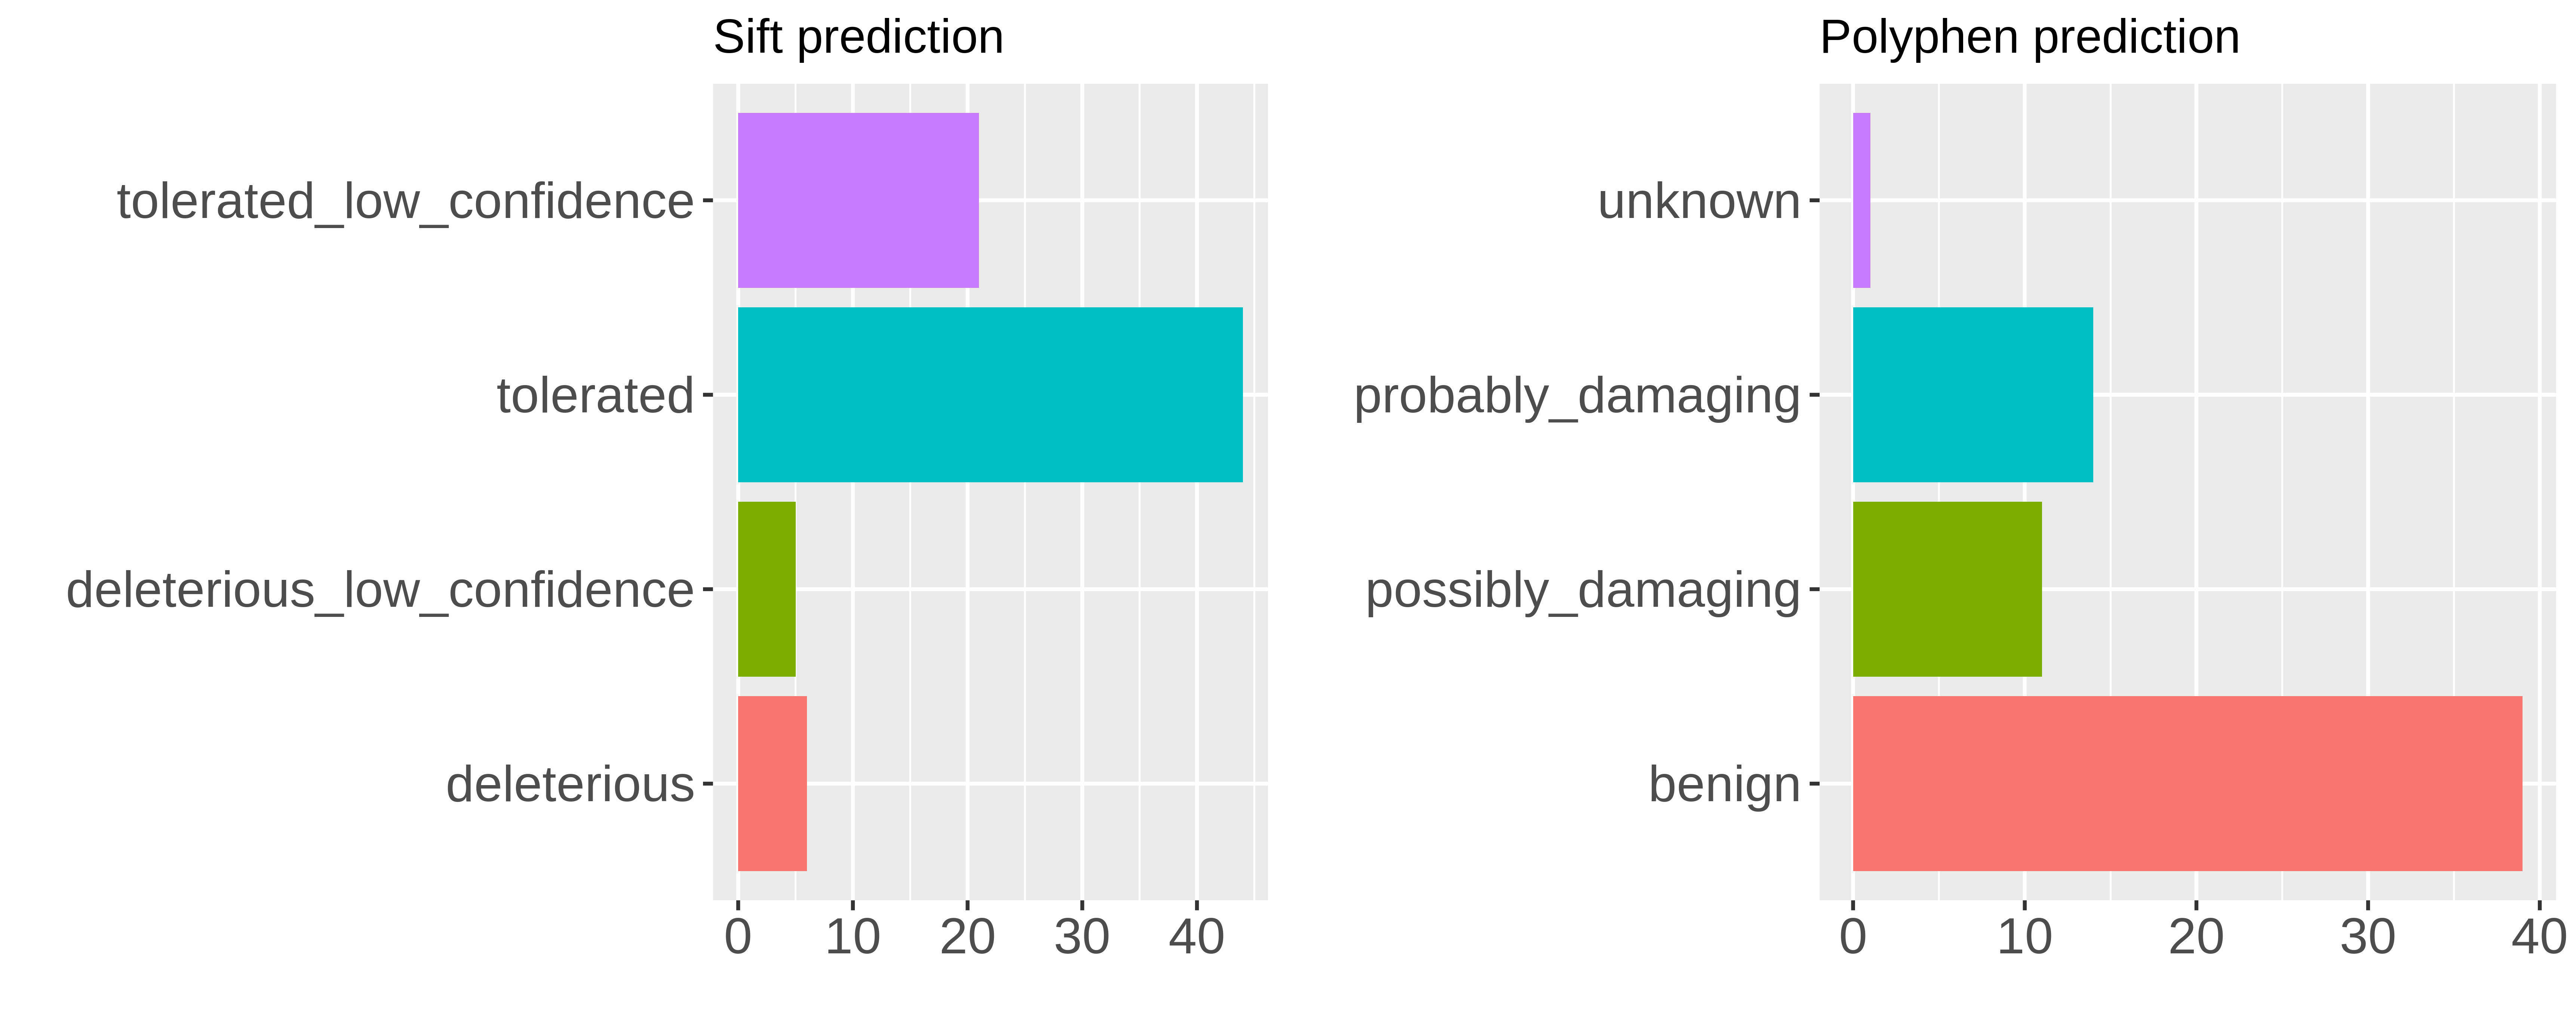
\includegraphics[width=1\textwidth]{Fig/nuclear_SiftPoly.png}
\caption{Sift and Polyphen Nuclear Gene}
\label{fig:siftpolyphen_nuclear}
\end{figure}\\



\newpage
\section{Heteroplasmy}

Mitochondrial heteroplasmy is defined as a dynamically determined co‐expression of wild type inherited polymorphisms and somatic mutations in varying ratios within individual mtDNA genomes distributed throughout the intraorganelle compartments of individual cells (\cite{stefano2016mitochondrial}).
Many of the pathogenic mtDNA mutations identified are heteroplasmic, especially the most severe ones. Heteroplasmic alleles can shift in percentage during both mitotic and meiotic cell division, this process is known as replicative segregation and could cause a potentially continuous array of bioenergetic defects. As the percentage of mutant mtDNAs increases, the resulting bioenergetic defect becomes increasingly severe. An example of the interaction between mtDNA heteroplasmy variation and phenotype was the report that the tRNA Lys nt 8344A.G  mutation that causes myoclonic epilepsy and ragged red fiber (MERRF) disease was heteroplasmic (\cite{wallace2013mitochondrial}). \\
The effect of mtDNA mutant heteroplasmy on phenotype is even more striking with the tRNA Leu(UUR) mt 3243A.G mutation associated with mitochondrial encephalomyopathy, lactic acidosis, and stroke-like episodes (MELAS, \cite{goto2011dynamics}). When the heteroplasmy of this mutation is high, it can present as lethal childhood Leigh syndrome, MELAS, chronic progressive external ophthalmoplegia (CPEO),cardiomyopathy, migraines, diabetes mellitus, and deafness. In pedigrees with high heteroplasmy members, meiotic segregation of the mutant mtDNAs can result in the full range of phenotypes from asymptomatic to lethal disease (\cite{wallace2013mitochondrial}).\\

To evaluate heteroplasmy in my data, I used \textsc{Mity - report} (\cite{puttick2019mity}). The file I obtained contains several parameters for determining heteroplasmy. Among the parameters the more relvant is of course the genotype. I considered genotypes reported as 0/1 as heteroplasmic variants. Among these, the percentage of heteroplasmy, i.e. the ratio between allele 1 and 0, varies from a minimum of 0.000100  to a maximum of 0.999900. When considering this whole range \textsc{Mity - report} identified 231 heteroplasmic sites in six embryos, as shown in Figure \ref{fig:distributionHet99}. When restricting the range of the ratio between the two alleles to  > 0.01 and < 0.90 the number of variants diminish as explained in figure \ref{fig:distribution90} \\ 

I have considered heteroplasmy in the four missense variants to determine any pathogenity linked to. (tab \ref{tab:missense}) \\



\begin{figure}[H]
\centering
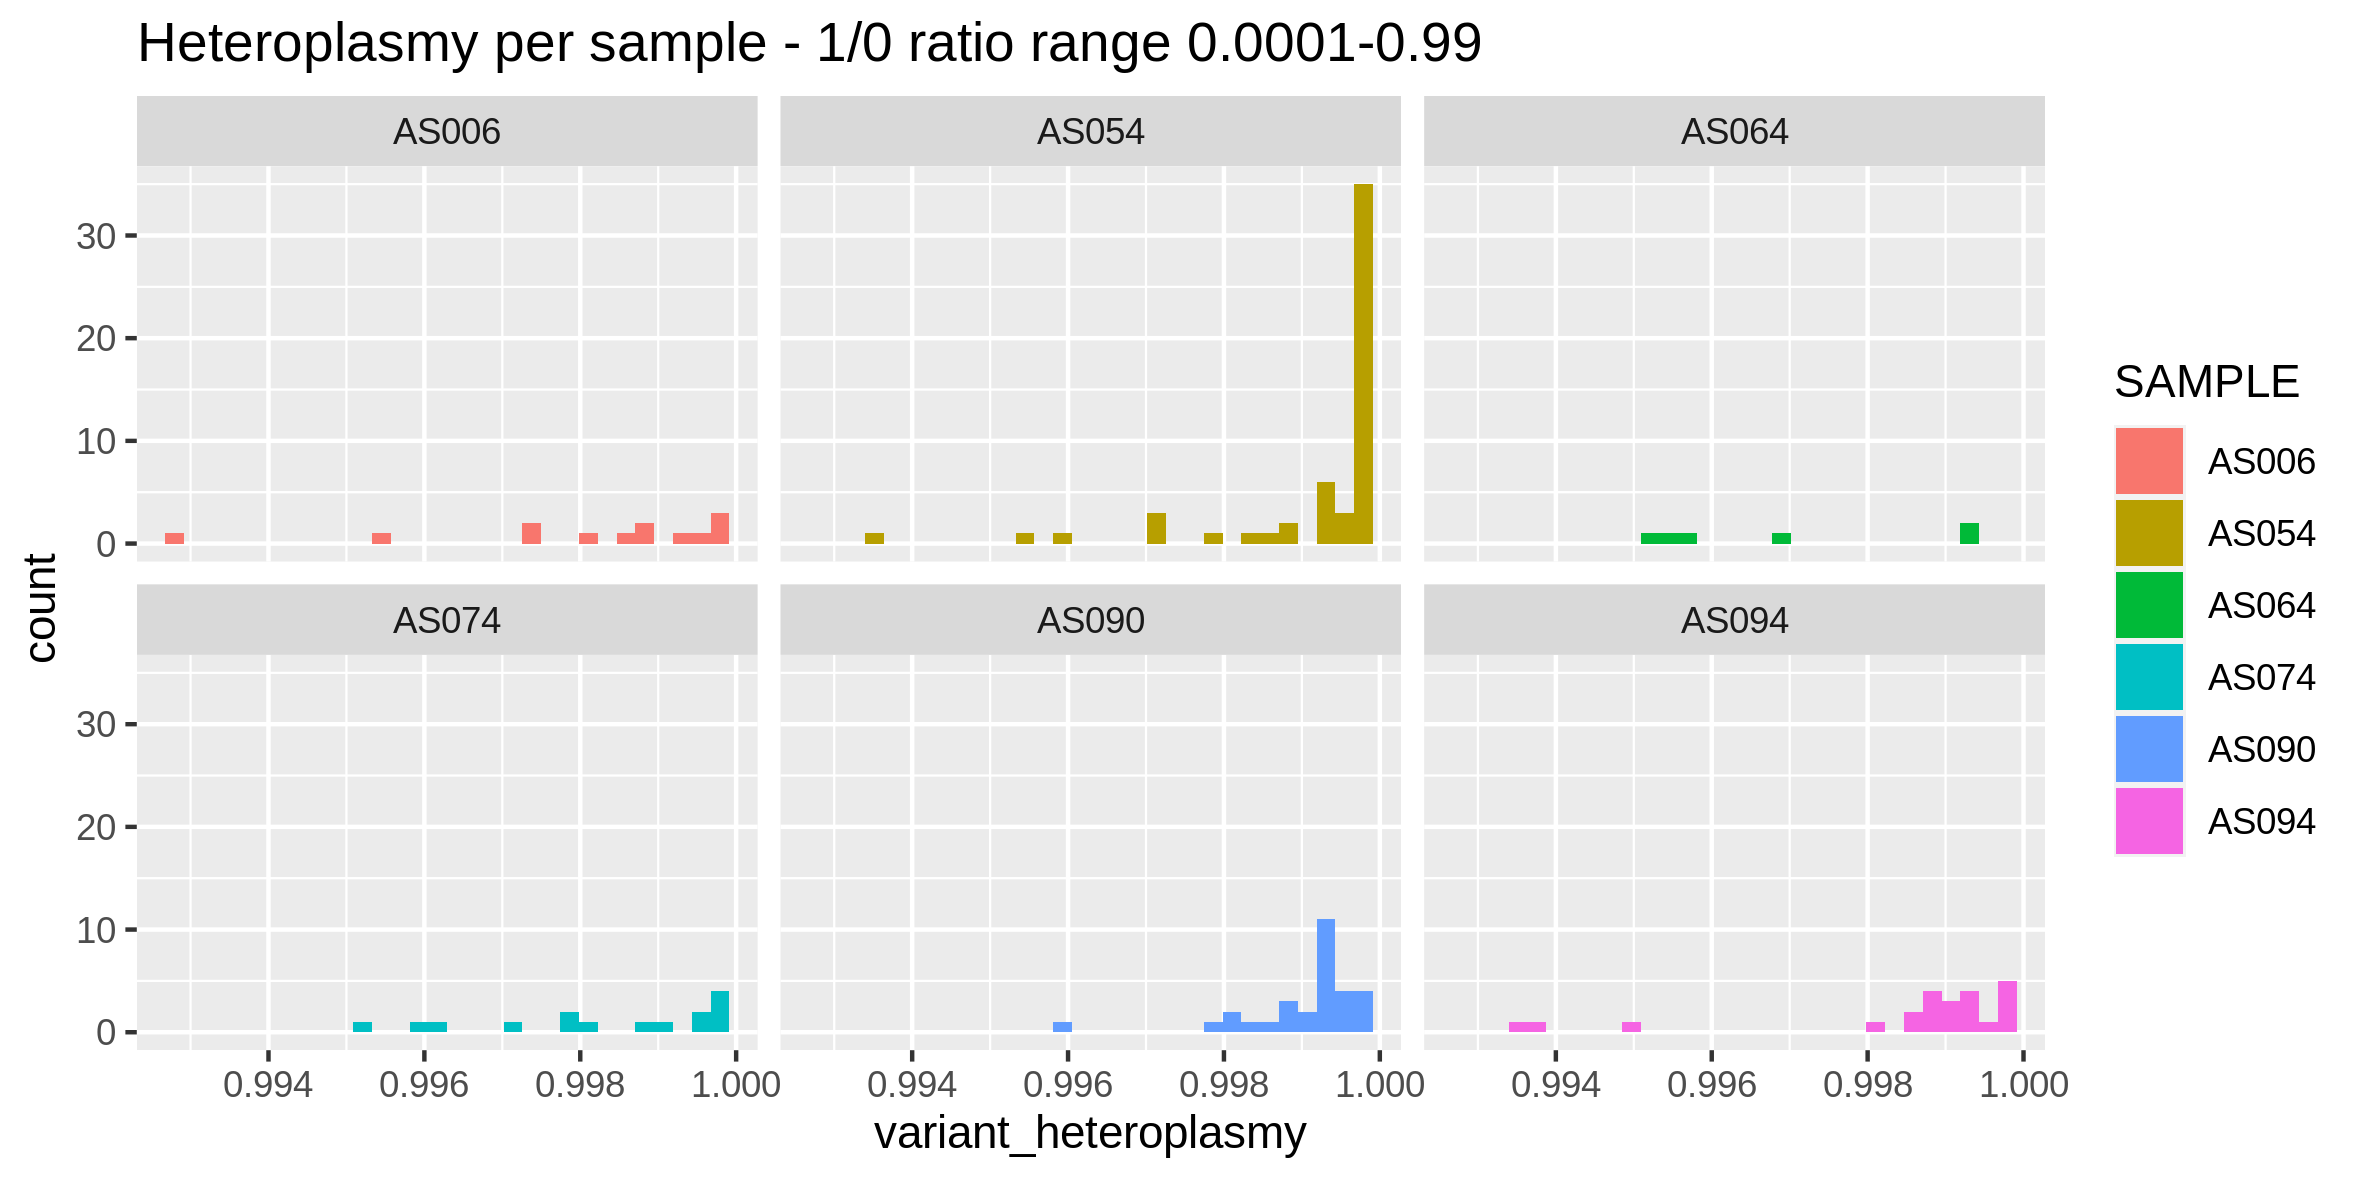
\includegraphics[width=1\textwidth]{Fig/het99.png}
\decoRule
\caption{\textbf{Heteroplasmy in the range of 0.000100 - 0.999900} Six embryos have heteroplasmic sites, y-axis indicate the counts and x-axis the percentage of heteroplasmy } 
\label{fig:distributionHet99}
\end{figure}


\begin{figure}[H]
\centering
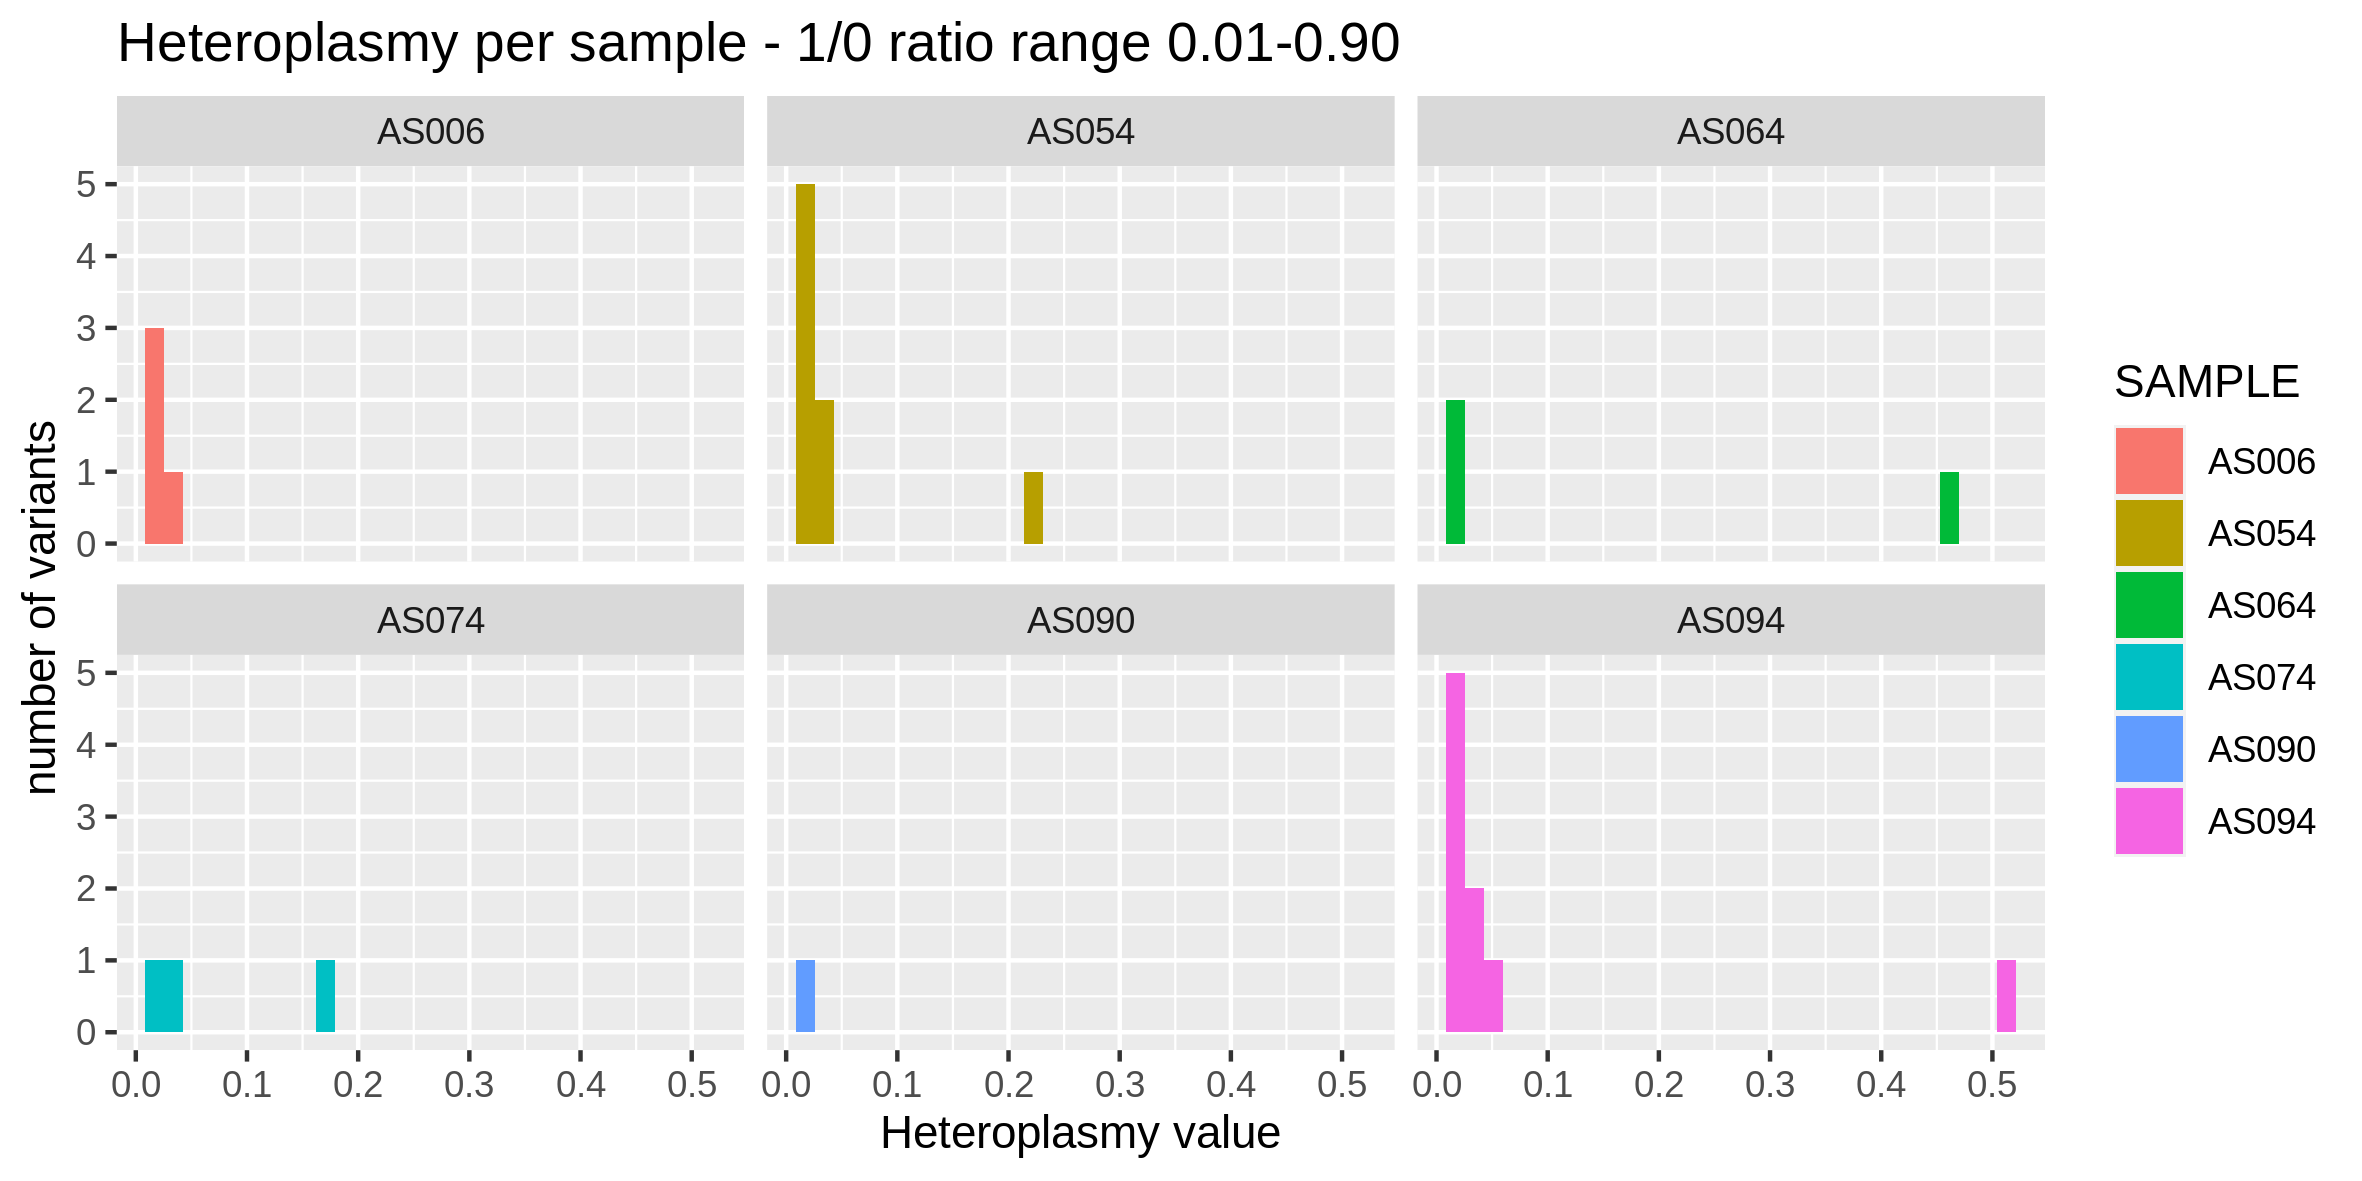
\includegraphics[width=1\textwidth]{Fig/het90.png}
\decoRule
\caption{\textbf{Heteroplasmy in the range of 0.01 - 0.90} Same as Figure \ref{fig:distributionHet99} but for a narrower range of heteroplasmy. y-axis indicate the counts and x-axis the percentage of heteroplasmy }
\label{fig:distribution90}
\end{figure}



\newpage
\section{Mitochondrial Haplogroups in the embryos }
The mtDNA can be classified into phylogenetic clusters, called Haplogroups.
Haplogroup is a group of similar haplotypes that share common ancestor, i.e. share some Single Nucleotide Polymorphism (SNP) mutations. It's called haplotype because it is only present in one chromosome of the pair, that is, in a haploid state. If a sufficient number of individuals are examined for their haplotypes, maps can be created, showing the distribution of haplogroups across the world. These maps are called Haplotype Maps (Figure \ref{fig:Haplogroups}), contain information about the order in which SNPs appeared through time, and they provide a variety of information, such as the ethnic makeup of a population, the history of past migrations of people to different parts of the world, etc. (\cite{arora2015hgsdb})\\
The regionality of the mtDNA haplogroups is important in several aspects. First, of all of the African diversity, only two mtDNA lineages (M and N) colonized the rest of the world. Second, of all of the Asian mtDNAs, only three mtDNA lineages (A, C, and D) moved to extreme northeast Siberia to found the Paleo-Indians. Third, the mtDNA sequence evolution rate is such that it produced important mtDNA evolutionary changes that coincide with the major human geographic migrations. Such associations could not have occurred by chance. Rather, it is most likely that mtDNA variation permitted adaptation of our human ancestors to different regional environments, thus being the adaptive system that permitted human colonization of the diverse environments that they encountered around the globe. (\cite{wallace2013mitochondrial})\\
To define the haplogroups in my data I used \textsc{Haplogrep}, a haplogroup classification tool (\cite{weissensteiner2016haplogrep}). The majority of sequences (n=8) belong to haplogroups H and T, typical of West Eurasia. One sequence belong to haplogroup L, typical of Africa, and two to haplogroups M and N which are commonly found in Asia. I was able to confirm the origin of the samples inferred by the haplogroups comparing it with the anthropometric records available.   
%My findings are concordant with the demographic data that were avaialble for these samples.  



{\small
\begin{table}[H]
\includegraphics[]{}
\caption{Haplogroups Location Tab}
\label{tab:Haplogroups}
\centering
\begin{tabular}{c c c c c c c}
\toprule
\tabhead{Geographic Location} & \tabhead{Haplogroup}\\
\midrule 
African &  L0, L1, L2, L3, L4, L5, L6   \\
West Eurasian & H, T, U, V, X, K, I, J, W.   \\
East Eurasian & A, B, C, D, E, F, G, Y, Z.\\
Native American & A, B, C, D, X \\
\bottomrule\\
\end{tabular}
\end{table}
}

{\small
\begin{table}[H]
\caption{Haplogroups}
\label{tab:Haplogroups}
\centering
\begin{tabular}{c c c c c c c}
\toprule
\tabhead{Sample ID} & \tabhead{Haplogroup} & \tabhead{Subgroup}\\
\midrule 
AS006 & H &  H2a2a   \\
AS030 & H &  H       \\
AS036 & H &  H7b1   \\
AS054 & L &  L1c3    \\
AS064 & H &  H+152    \\
AS065 & N &   N1a1    \\
AS074 & H &   H+152   \\
AS087 & M & M5a2a1a1   \\
AS090 & T &  T2b3+151  \\
AS093 & T &   T2c1   \\
AS094 & H &    H     \\
\bottomrule\\
\end{tabular}
\end{table}
}



\begin{figure}[H]
\centering
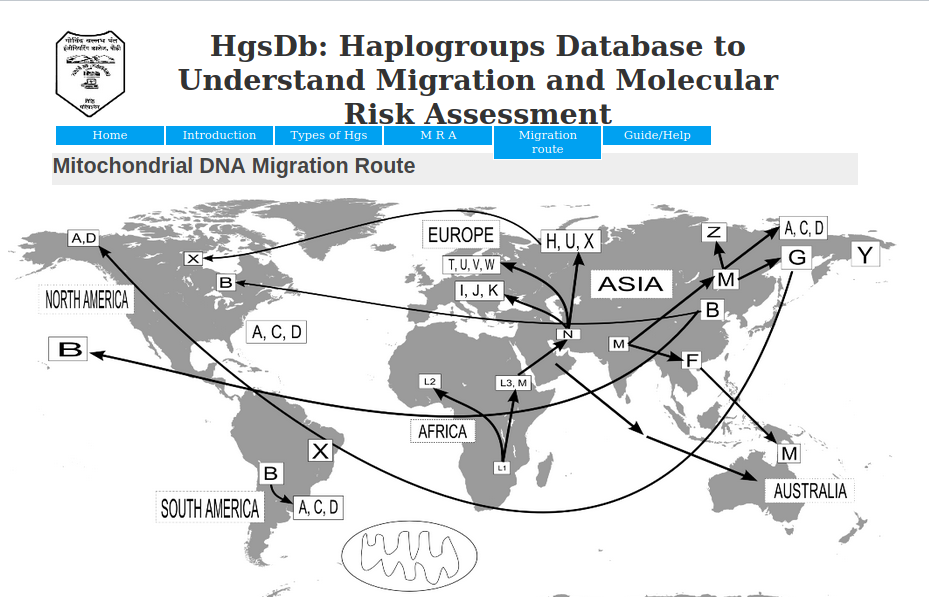
\includegraphics[width=1\textwidth]{Fig/HaplogroupsMigration.png}
\decoRule
\caption{\textbf{}} \textit{ Adapted from \cite{arora2015hgsdb}}. 
\label{fig:Haplogroups}
\end{figure} 

%\begin{figure}[H]
%\centering
%\includegraphics[width=\textwidth]{Fig/MtDNA_haplogroup_tree_and_di%stribution_map.png}
%\decoRule
%\caption{\textbf{}} \textit{ Adapted from %\cite{kivisild2015maternal}}. 
%\label{fig:Haplogroups}
%\end{figure} 